%  -----------------------------------------------------------------------------
%  -----------------------------------------------------------------------------
%  Numerical simulation of bubble deformation and breakup under simple linear 
%  shear flows
%  
%  Authors: Mitsuhiro Ohta, Tetsuya Ueta, Yozo Toei, Edwin Jimenez, and
%           Mark Sussman
%  
%  Modified: 22 December 2022
%  -----------------------------------------------------------------------------
%  -----------------------------------------------------------------------------

% ****** Start of file apssamp.tex ******
%
%   This file is part of the APS files in the REVTeX 4.2 distribution.
%   Version 4.2a of REVTeX, December 2014
%
%   Copyright (c) 2014 The American Physical Society.
%
%   See the REVTeX 4 README file for restrictions and more information.
%
% TeX'ing this file requires that you have AMS-LaTeX 2.0 installed
% as well as the rest of the prerequisites for REVTeX 4.2
%
% See the REVTeX 4 README file
% It also requires running BibTeX. The commands are as follows:
%
%  1)  latex apssamp.tex
%  2)  bibtex apssamp
%  3)  latex apssamp.tex
%  4)  latex apssamp.tex
%
\documentclass[%
 reprint,
 showkeys,
%superscriptaddress,
%groupedaddress,
%unsortedaddress,
%runinaddress,
%frontmatterverbose, 
%preprint,
%preprintnumbers,
%nofootinbib,
%nobibnotes,
%bibnotes,
 amsmath,amssymb,
 aps,
 prfluids,
 onecolumn
%prfluids,
%pra,
%prb,
%rmp,
%prstab,
%prstper,
%floatfix,
]{revtex4-2}

\usepackage{graphicx}% Include figure files
\usepackage{dcolumn}% Align table columns on decimal point
\usepackage{bm}% bold math
%\usepackage{hyperref}% add hypertext capabilities
%\usepackage[mathlines]{lineno}% Enable numbering of text and display math
%\linenumbers\relax % Commence numbering lines

%\usepackage[showframe,%Uncomment any one of the following lines to test 
%%scale=0.7, marginratio={1:1, 2:3}, ignoreall,% default settings
%%text={7in,10in},centering,
%%margin=1.5in,
%%total={6.5in,8.75in}, top=1.2in, left=0.9in, includefoot,
%%height=10in,a5paper,hmargin={3cm,0.8in},
%]{geometry}

\graphicspath{{figures/}}
\setlength{\tabcolsep}{12pt} % Modifies table column separation.

% MATH -------------------------------------------------------------------------
\newcommand{\Hea}{\mathcal{H}}
\newcommand{\opI}{\mathcal{I}}

\newcommand{\N}{\mathbb{N}}
\newcommand{\R}{\mathbb{R}}
\newcommand{\C}{\mathbb{C}}
%\newcommand{\Real}[1]{\text{Re}\left\{#1\right\}}
%\newcommand{\Imag}[1]{\text{Im}\left\{#1\right\}}

\newcommand{\eps}{\epsilon}
\newcommand{\veps}{\varepsilon}
\newcommand{\ep}{\varepsilon}
\newcommand{\ome}{\omega}

\newcommand{\del}{\partial}
%\newcommand{\Bdy}{\del\Dom}
%\newcommand{\dive}{\nabla\cdot}
%\newcommand{\divS}{\text{div}_{\Bdy}}

\newcommand{\vv}{\mathbf}
\newcommand{\bmD}{\vv{D}}
\newcommand{\bmg}{\vv{g}}
\newcommand{\bmI}{\vv{I}}
\newcommand{\bmu}{\vv{u}}

\newcommand{\LWH}{L\times W \times H}

%\newcommand{\twoFigWidth}{0.485}

\newcommand{\lwh}[3]{L(#1R)\times W(#2R) \times H(#3R)}
%\newcommand{\dist}[1]{\text{dist}\left(#1\right)}
%\newcommand{\jump}[1]{\left[#1\right]_{-}^{+}}
%\newcommand{\norm}[1]{\left\Vert#1\right\Vert}
%\newcommand{\abs}[1]{\left\vert#1\right\vert}
%\newcommand{\floor}[1]{\left\lfloor#1\right\rfloor}
%\newcommand{\ceil}[1]{\left\lceil#1\right\rceil}
%
%\newcommand{\vnu}{\boldsymbol\nu}
%\DeclareMathOperator*{\argmax}{arg\,max}
%\DeclareMathOperator*{\argmin}{arg\,min}

%  -----------------------------------------------------------------------------
\begin{document}

%\preprint{APS/123-QED}

%\title{Manuscript Title:\\with Forced Linebreak}% Force line breaks with \\
%\thanks{A footnote to the article title}%
\title{Numerical simulation of bubble deformation \\
       and breakup under simple linear shear flows}

\author{Mitsuhiro Ohta}
 \altaffiliation[Also in the ]{Department of Mechanical Engineering, Graduate School 
                 of Advanced Technology and Science,
                 Tokushima University}%Lines break automatically or can be forced with \\
  \email{m-ohta@tokushima-u.ac.jp}
\affiliation{
  Department of Mechanical Science, Graduate School of Technology, Industrial and Social Sciences,
  Tokushima University,\\
  2-1 Minamijyousanjima-cho,Tokushima 770-8506, Japan}
\author{Tetsuya Ueta}
\affiliation{
   Department of Mechanical Engineering, Graduate School of Advanced Technology and Science,\\
  Tokushima University, 2-1 Minamijyousanjima-cho,Tokushima 770-8506, Japan}
\author{Yozo Toei}
 %\email{Second.Author@institution.edu}
\affiliation{%
 %Authors' institution and/or address\\
 %This line break forced with \textbackslash\textbackslash
 High Performance Plastics Company, Sekisui Chemical Co., Ltd.,\\
 2-1 Hyakuyama, Mishimagun Shimamoto-cho, Osaka 618-0021, Japan
}%

%\collaboration{MUSO Collaboration}%\noaffiliation

\author{Edwin Jimenez}  
\affiliation{Department of Computing and Mathematical Sciences, MC 305-16 
             California Institute of Technology, Pasadena, CA 91125, USA
}%

\author{Mark Sussman}  
\affiliation{
  Department of Mathematics,
  Florida State University,
  Tallahassee, FL 32306, USA
}%

%\collaboration{CLEO Collaboration}%\noaffiliation

\date{\today}% It is always \today, today,
             %  but any date may be explicitly specified

\begin{abstract}
Numerical simulations for the deformation and breakup of a bubble in liquids
undergoing simple linear shear flow are presented.  Computational results are
obtained using a hydrodynamic scheme with formal second-order accuracy based on
a coupled level set/volume-of-fluid (CLSVOF) method.  To verify our numerical
algorithm, and to provide a basis for comparison, we also present simulation
results which compare with previous, more popular, simulations  
of drop deformation and rupture.  The numerical
results reveal that the shear-induced bubble deformation and breakup process
differs significantly from that of the analogous drop system under similar flow
conditions.  The first distinguishing factor for bubble breakup is that the
magnitude of shear flow necessary for rupture is much larger than that in the
drop system case.  In other words, a larger Reynolds number is necessary to
induce bubble breakup.  The second distinct feature of the bubble system versus
the drop system is that the bubble does not maintain a stable deformed shape as
the parameters of the system approach the critical ``breakup'' Reynolds number.
It is asserted that the differences in morphology for a bubble undergoing
breakup, versus a drop in the same process, can be attributed to the density
and viscosity ratio of the corresponding two-phase flow systems.  The critical
conditions for bubble breakup with respect to the Reynolds and capillary
numbers are determined for several cases.
\end{abstract}

%\keywords{Suggested keywords}%Use showkeys class option if keyword
%                              %display desired
\keywords{Bubble deformation, bubble breakup, shear flow, CFD}

\maketitle

%\tableofcontents

%  -----------------------------------------------------------------------------
\section{Introduction}
%  -----------------------------------------------------------------------------

%
% Note: There were missing references in the .bib file for the following cite tags: 
%       WanMacReni02, OlaSinSak09, ZhaBag11, BayMor11, and Ren08-1. 
%       (Edwin, April 29, 2022)
%
The study of the deformation and breakup of a drop in immiscible viscous
liquids undergoing simple linear shear flow has been investigated extensively
due to its fundamental importance in connection with emulsion and materials
processing, mixing and reaction devices. The pioneering experimental work
of this problem was performed by Taylor in the early 1930s \cite{Tay32, Tay34},
and the subsequent theoretical and experimental progress up to the 1980s and
1990s was reviewed in \cite{Ral84} and \cite{Sto94}, respectively.  By the
2000s, progress in computational fluid dynamics (CFD) techniques and increased
access to powerful computing resources led to a surge of research focused on
direct simulations of this problem.  In particular, detailed computational
investigations of drop breakup, 
based on a Volume-of-Fluid (VOF) method \cite{HirNic81} were
presented in \cite{LiRenRen00, RenCri01-1, RenCri01-2, RenCriLi02,
KhiRenCri03,Ren06,Ren07,Ren08-2}.  Since then, the literature on computational
studies on the deformation and breakup of a single or several drops in shear
flow has continued to grow \cite{CriGuiAlfBlaLoe03, InaTomOgi03,ZhaMikBan06,
BazAndMei06, JanAnd08, CroGriSch10,KomShaEskDer14,KomShaEskDer15, IoaLiuZha16,
HerRan17,AmaBalCasOli19, ZhaShuGuaYan21} and a variety of numerical techniques
have been developed to tackle this problem, including boundary-integral
approaches \cite{CriBlaLoe01, JanAnd07}, lattice Boltzmann methods \cite{Ina06,
KomShaEskDer14}, front tracking schemes \cite{UnvTry92}, and interface-tracking
level set methods \cite{SusSmeOsh94}.  

In contrast, few computational studies on bubble deformation and breakup in
shear flow have been conducted \cite{WanShiZha15}.  This type of bubble
dynamics in shear flow is of critical importance for a variety of
scientific and engineering processes. We refer the reader to the 
following experimental studies relating to bubble deformation in foaming
processes, microfluidic devices, and micro bubbles in the blood 
circulation system,
\cite{CHU2019108,muller2008single,bento2018deformation,drenckhan2015science}.
In particular, it is the study of bubble deformation as it pertains
to high performance plastics applications which motivates this work.  
In this article, we present
computational studies of shear-driven deformation and breakup of a bubble in
insoluble viscous liquids.  
Studying bubble break-up via computation rather
than experiments simplifies the process of setting a combination of
precise simple shear flow conditions, low $Ca$ conditions, low density ratio, 
and low viscosity ratios.
The physical properties that distinguish bubble and
drop studies are expressed in terms of the density ratio $\lambda = \rho_b /
\rho_m$ and the viscosity ratio $\eta = \mu_b / \mu_m$, where $\rho$ is the
fluid density, $\mu$ is the viscosity and the subscripts ``b'' and ``m'' denote
the ``bubble'' or ``drop'' and the ``matrix fluid'', respectively.  For a
bubble in an insoluble viscous liquid, the density ratio $\lambda \simeq 0$ and
the viscosity ratio $\eta \simeq 0$, whereas most studies dealing with a drop
in an immiscible viscous liquid take $\lambda =1$ and $\eta \simeq 1$.  

In this work we focus on identifying critical flow states numerically, in terms
of dimensionless quantities, that specify the extreme conditions at which a
bubble or drop in shear flow first transitions from deformation to breakup.
We validate our numerical method through comparisons with previous
shear-driven drop dynamics results and we also examine the effect of drop
deformation and breakup sensitivity on domain and grid size.  An advantage of
studying shear-driven bubble deformation and breakup computationally, rather
than experimentally, is that we can easily modify fluid physical properties to
ascertain the sensitivity of deformation and breakup to physical parameters.
In our computations, the time-evolution of the boundary between gas and liquid
is tracked with a coupled level set/volume-of-fluid (CLSVOF) interface
capturing algorithm \cite{SusPuc00}.  We focus on determining critical physical
conditions in which the breakup of a bubble occurs in shear flow because it is
important to identify the parameter regimes in which a relatively simple system
transitions from stable to unstable.  Specifically, we identify the critical
Reynolds number $Re_{c}$ corresponding to the bubble breakup onset condition as
a function of the Capillary number $Ca$.  The critical Reynolds number, 
$Re_{c}$, for drop
breakup was reported previously \cite{LiRenRen00}, in this work we determine,
for the first time, the critical Reynolds number that leads to \emph{bubble}
breakup.  Additionally, our computational studies reveal characteristics that
distinguish the deformation and breakup processes of a drop versus those of a
bubble.


%  -----------------------------------------------------------------------------
\section{Problem Description}
%  -----------------------------------------------------------------------------

Figure~\ref{fig:SchemAndGrid}(a) shows a schematic of the computational system
for our studies of a bubble (or drop) in shear flow.  The computational domain
consists of a three-dimensional rectangular domain of $L(x)$ (length) $\times$
$W(y)$ (width) $\times$ $H(z)$ (height).  The size of $L(x)$, $W(y)$ and $H(z)$
was determined after consideration of numerical result sensitivity to domain
size; numerical studies of domain-size dependence are presented in
Section~\ref{sec:DomGrdSize}.  All computational results that follow were
obtained from numerical solutions of the three-dimensional governing equations
for gas-liquid/liquid-liquid flows.  Computations are initialized with a
spherical bubble set at the center of the domain that is then subjected to a
linear shear flow generated by the motion of the top and bottom plates, which 
have constant velocity $+V$ and $-V$, respectively.  In the interior of the
domain, the initial velocity condition is assumed to be a simple linear profile
and periodic boundary conditions are imposed along the $x$ and $y$ directions.
Mathematically, the initial and boundary conditions are described as
follows:
\begin{eqnarray}
	\phi(x,y,z,0)=\sqrt{(x-\frac{L}{2})^{2}+(y-\frac{W}{2})^{2}+
	(z-\frac{H}{2})^{2}}-R \label{IC_BC} \\
	\bmu(x,y,z,0)=\left( \begin{array}{c}
		\frac{2V}{H}(z-\frac{H}{2}) \\ 0 \\ 0 
	\end{array} \right) \nonumber \\
	\phi(x+L,y,z,t)=\phi(x,y,z,t) \hspace{20pt}
	\phi(x,y+W,z,t)=\phi(x,y,z,t) \nonumber \\
	\bmu(x,y,H,t)=\left( \begin{array}{c}
		                V \\ 0 \\ 0 
	\end{array} \right)  \hspace{20pt}
	\bmu(x,y,0,t)=\left( \begin{array}{c}
		                -V \\ 0 \\ 0 
	\end{array} \right)  \nonumber \\
	\bmu(x+L,y,z,t)=\bmu(x,y,z,t) \hspace{20pt} 
	\bmu(x,y+W,z,t)=\bmu(x,y,z,t). \nonumber
\end{eqnarray}
$\phi(x,y,z,t)$ is a material indicator function which is positive 
in the ``matrix'' fluid and negative in the bubble (or drop) fluid.
$\bmu(x,y,z,t)$ is the velocity.

Common dimensionless physical parameters used to describe gas-liquid or
liquid-liquid two-phase flows include the Reynolds ($Re$), Weber ($We$) (or
$Ca$ (= $We/Re$)) and Froude ($Fr$) numbers, and the density ratio $\lambda$
and viscosity ratio $\eta$.  For comparison with previous drop studies, we set
$\lambda=1$ and, since in this case the effect of gravity is not considered, we
may ignore the Froude number $Fr$.  As a result, (for $\lambda=1$) the
following dimensionless physical parameters are used to describe the problem of
drop or bubble deformation/breakup in shear flow
%
\begin{eqnarray}\label{dimensonless}
  Re = \frac{\rho_{b}UR}{\mu_{b}}, \quad
  Ca = \frac{\mu_{b}U}{\sigma}, \quad
  \eta = \frac{\mu_{b}}{\mu_{m}}
\end{eqnarray} 
%
where $R$ is the drop or bubble radius, $\sigma$ denotes the surface tension,
and $U$ is the velocity scale. For the problem of shear-induced drop
deformation and breakup, the velocity is set to $U = \mathit{\Gamma} R$, where
the shear-rate $\mathit{\Gamma} = 2V/H$.  As mentioned in the introduction,
most previous drop studies set $\eta = 1$. Thus, for comparison, in this case
we will set $\lambda = \eta = 1$ (and also neglect the effect of gravity so
that $g=0$). On the other hand, in our computations for a bubble, we set the
density and viscosity of air to $\rho_{b}$ = 1.2 kg/m$^{3}$ and $\mu_{b}$ = 1.8
$\times$ $10^{-5}$ Pa$\cdot$s, and we take the 
density ratio 
%%$\lambda$ = 1.2 $\times$ $10^{-3}$ 
$\lambda$ = 1.0 $\times$ $10^{-3}$ 
and the 
viscosity ratio 
%%$\eta$ $<$ 1.0 $\times$ $10^{-3}$.
$\eta$ $=$ 1.0 $\times$ $10^{-3}$.
For consistency with previous studies, we will computationally examine the
deformation and breakup of a bubble in simple linear shear flow as a
function of $Re$ and $Ca$ numbers.  In particular, 
for a certain $Ca$ value, we
focus on determining the critical value 
$Re_{c}$ that corresponds to the threshold
for breakup.

%  -----------------------------------------------------------------------------
\section{Numerical Analysis}
%  -----------------------------------------------------------------------------
% 
\begin{figure}%[h!]
  \centering
  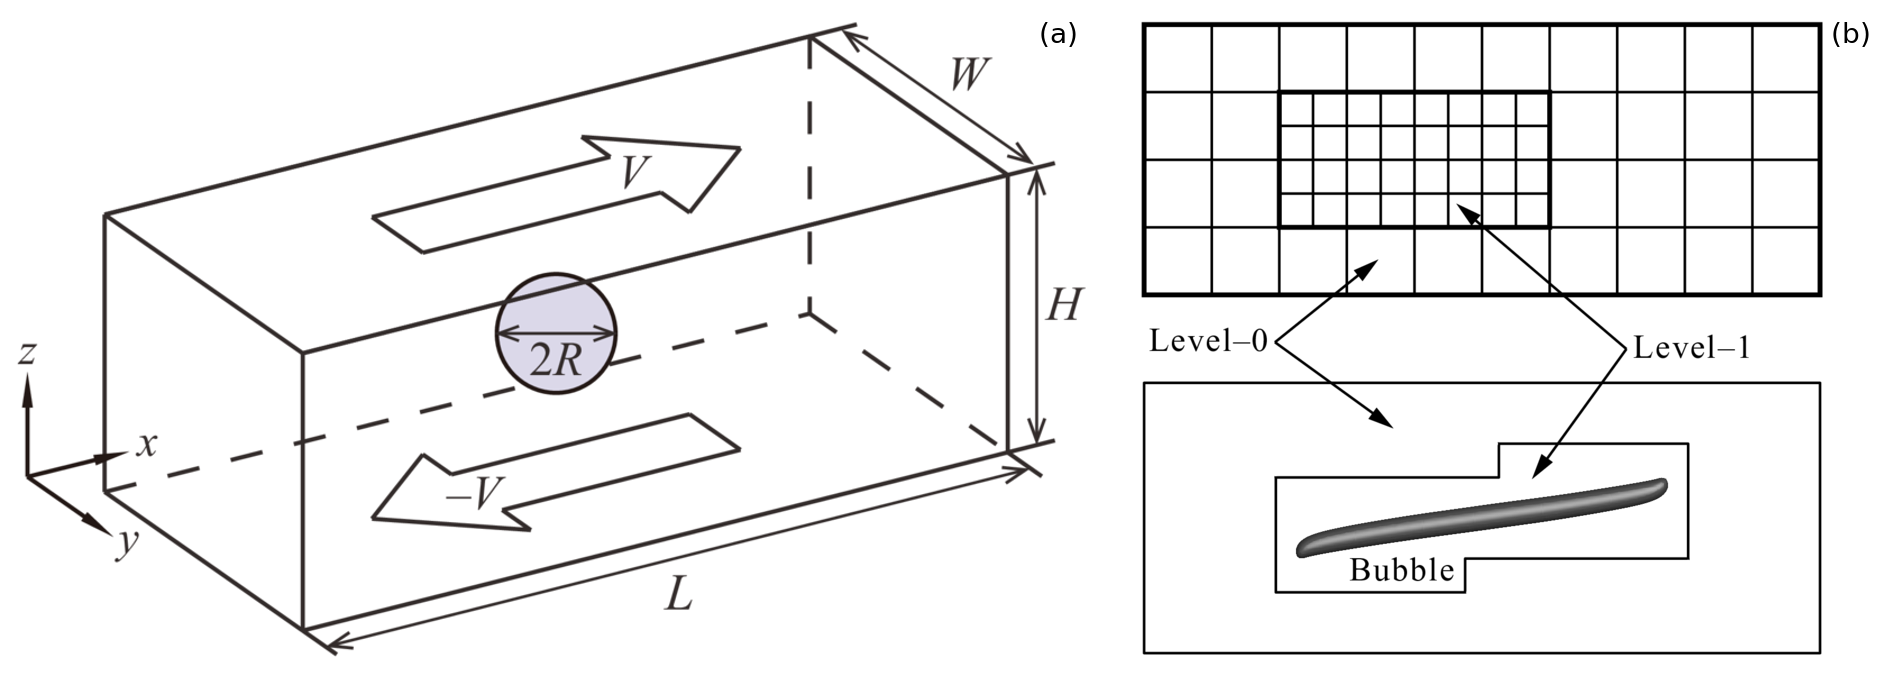
\includegraphics[width=\textwidth]{SchematicAndGrid}
  \caption{(a) Computational domain schematic for a bubble or drop in shear 
           flow and (b) (\textit{upper panel}) a two-level adaptive mesh 
           refinement (AMR) grid schematic with an actual computational 
           example (\textit{lower panel}) of bubble deformation in simple linear 
           shear flow.}
  \label{fig:SchemAndGrid}
\end{figure}
%

\subsection{Numerical method and governing equations}
%  -----------------------------------------------------------------------------
Numerical results were obtained using the interface-tracking CLSVOF method,
which is based on a fixed grid finite volume algorithm.  In our studies,
the two-phase fluid flow is comprised of air and a 
viscous Newtonian liquid.  The
Heaviside function, $\Hea(\phi)$, which is defined as
%
\begin{equation}\label{heavyeqn}
  \Hea(\phi) = \begin{cases}
               1 & \phi \geq 0 \\
               0 & \phi <0 
               \end{cases}
\end{equation}
%
will be used below to distinguish each of the two fluids.  A single set of
three-dimensional equations governs the motion of both fluids, which are taken
to be incompressible, and consists of the continuity equation and the
Navier-Stokes equations with surface tension forces:
%
\begin{align}
  \nabla\cdot\bmu &=0  \label{divu} \\
  \frac{\partial\bmu}{\partial t}+(\bmu\cdot\nabla)\bmu &=
  \frac{1}{\rho}\nabla\cdot(-p\bmI+2\mu\bmD)+\bmg-
  \frac{\sigma\kappa}{\rho}\nabla \Hea  \label{nseqn}
\end{align}
%
%%
%\begin{eqnarray}
%\nabla\cdot\bmu=0  \label{divu} %\\
%\end{eqnarray}
%%
%\begin{eqnarray}
%\frac{\partial\bmu}{\partial t}+(\bmu\cdot\nabla)\bmu=
%\frac{1}{\rho}\nabla\cdot(-p\bmI+2\mu\bmD)+\bmg-
%\frac{\sigma\kappa}{\rho}\nabla H  \label{nseqn}
%\end{eqnarray}
%
where $\bmu$ is the velocity vector, $t$ represents time, $p$ is the pressure,
$\bmI$ is the unit tensor, $\bmD$ is the rate of deformation tensor
($\bmD=\frac{1}{2}(\nabla\bmu+(\nabla\bmu)^{T})$), $\rho$ is the density, $\mu$
is the viscosity, $\kappa$ is the interfacial curvature, and the Heaviside
function $\Hea(\phi)$ is a function of the level set (LS) function $\phi$. The
singular Heaviside gradient term in the right hand side of
equation~\eqref{nseqn} is a body force representing the surface tension force
and is equivalent
to specifying that the jump in the normal stress is equal to
$\sigma\kappa$~\cite{TanguyEtAl2007}.  The interfacial curvature $\kappa$ is
computed with second order accuracy directly from the volume-of-fluid (VOF)
function using the height function technique~\cite{sussman2003second}.  
We remark that we get the same
results if we were to compute $\kappa$ directly from the LS function using the
``level set'' height function technique.

Since $\rho$ and $\mu$ are taken to be constant in each fluid, with a jump at
the interface, they can be expressed in terms of the Heaviside function,
%
\begin{eqnarray}\label{rhomu}
  \rho=\rho_{\rm m}\Hea+\rho_{\rm b}(1-\Hea), \qquad 
  \mu=\mu_{\rm m}\Hea+\mu_{\rm b}(1-\Hea).
\end{eqnarray}
%
The subscripts ``b'' and ``m'' refer to ``drop or bubble'' and ``matrix
fluid'', respectively. To represent the free surface with the CLSVOF method, we
must evolve the solution to both the VOF equation for $F$ and the LS equation
for $\phi$:
%
%\begin{subequations}\label{eq:clsvof}
\begin{align}\label{eq:clsvof}
  \frac{\partial F}{\partial t}+(\bmu\cdot\nabla)F = 0, \qquad 
  \frac{\partial \phi}{\partial t}+(\bmu\cdot\nabla)\phi = 0. 
\end{align}
%\end{subequations}
%
In all computations the discretized variables $p$, $\phi$ and $F$ are located at
cell centers and the discrete variable $\bmu$ is located at cell face centers.
Our computations are performed using an overall second-order accurate
hydrodynamic scheme.  The spatial discretization uses second-order accurate,
slope-limited, upwind techniques for the nonlinear advective terms.  The
velocity and pressure fields are computed using an implicit pressure projection
procedure. 

To make efficient use of computational resources, our numerical simulations
utilize an adaptive hierarchy of grids based on a dynamic adaptive mesh
refinement (AMR) technique~\cite{SusAlmBelColHowWel99}.  Adaptive grids are
dynamically adjusted based on the location of the 
deforming gas-liquid interface.
In the AMR technique the grid resolution is increased in regions near the
interface while a coarser grid is used where the flow is relatively steady.
The upper panel of Figure~\ref{fig:SchemAndGrid}(b) displays a schematic view
of the hierarchical grid structure and the lower panel corresponds to an actual
computational example for bubble deformation in simple linear shear flow.  In
general, the mesh hierarchy is composed of different levels of refinement
ranging from coarsest $\ell=0$ (``level-0") to finest
$\ell=\ell_{\textrm{max}}$ (``level-$\ell_{\textrm{max}}$").  The refinement
ratio of one grid size ($\Delta x=\Delta y=\Delta z$) to the next finer level
is two so that $\Delta x^{\ell+1}=0.5\Delta x^{\ell}$.  All computations in
this study used an AMR system with a maximum prescribed level
$\ell_{\textrm{max}} = 1$ (as illustrated in the upper panel of
Figure~\ref{fig:SchemAndGrid}(b)).  In our adaptive mesh refinement algorithm,
the velocity in coarse grid cells that neighbor fine grid cells is interpolated
from the coarse grid using bilinear interpolation in order to initialize
``ghost'' fine cells. Thus, the bilinear interpolation procedure produces
interpolated fine grid data as a linear combination of the coarse grid data. 

\subsection{Validation of the numerical method}
%  -----------------------------------------------------------------------------
Numerical studies reported in this section
are presented in order to verify the accuracy of our computational
method.  First, we compare quantitatively against the steady-state drop
deformation results reported by Li et al.~\cite{LiRenRen00}.  The shape of a
deformed drop in simple linear shear flow is described in terms of the Taylor
deformation parameter $De=(a-b)/(a+b)$, where $a$ and $b$ are the major and
minor axes of the deformed drop.  For consistency, we perform numerical
simulations using CLSVOF over the same computational domain and grid size used
in~\cite{LiRenRen00}, which has dimensions $\lwh{8}{4}{8}$ (recall that $R$ is
the bubble/drop radius) and a level-0 grid size $\Delta x=\Delta y=\Delta
z=R/8$; our two-level AMR grid structure also uses a finer level-1 grid size
$\Delta x^{\ell=1} = \Delta y^{\ell=1} = \Delta z^{\ell=1} = R/16$.  Numerical
results are listed in Table~\ref{tab:DeComparison} for $De$ as a function of
$Re$, with $Ca=0.3$ and $\lambda = \eta = 1$ fixed in every case, obtained with
the VOF method used in \cite{LiRenRen00}, and also with our CLSVOF algorithm.
Table~\ref{tab:DeComparison} indicates that our numerical results are in good
agreement with previous computations for drop deformation and breakup.
%
\begin{table}[tbh]
\caption{Comparison of the Taylor deformation parameter $De$ for a drop as a function 
         of $Re$ ($Ca=0.3$, $\lambda = \eta = 1$). In all cases, the domain 
         size is $\lwh{8}{4}{8}$, where $R$ is the drop radius.
         CLSVOF method computations used a two-level AMR computational domain 
         with a level-0 discretization $\Delta x^{\ell=0} = \Delta y^{\ell=0} 
         = \Delta z^{\ell=0} = R/8$ and a level-1 discretization
         $\Delta x^{\ell=1} = \Delta y^{\ell=1} = \Delta z^{\ell=1} = R/16$.}
\label{tab:DeComparison}
%\footnotesize
\center
\begin{tabular}{ c  c  c  c  c }
\hline
\hline
Reynolds number                      & 0.1     & 0.5     & 0.6     & 0.75      \\
$De$(Li et al. (\cite{LiRenRen00}))  & 0.3968  & 0.45    & 0.4768  & Breakup   \\
$De$(Our study)                      & 0.3960  & 0.4570  & 0.4758  & Breakup   \\
\hline
\hline
\end{tabular}
\end{table}
%
\begin{figure}[h!]
  \centering
  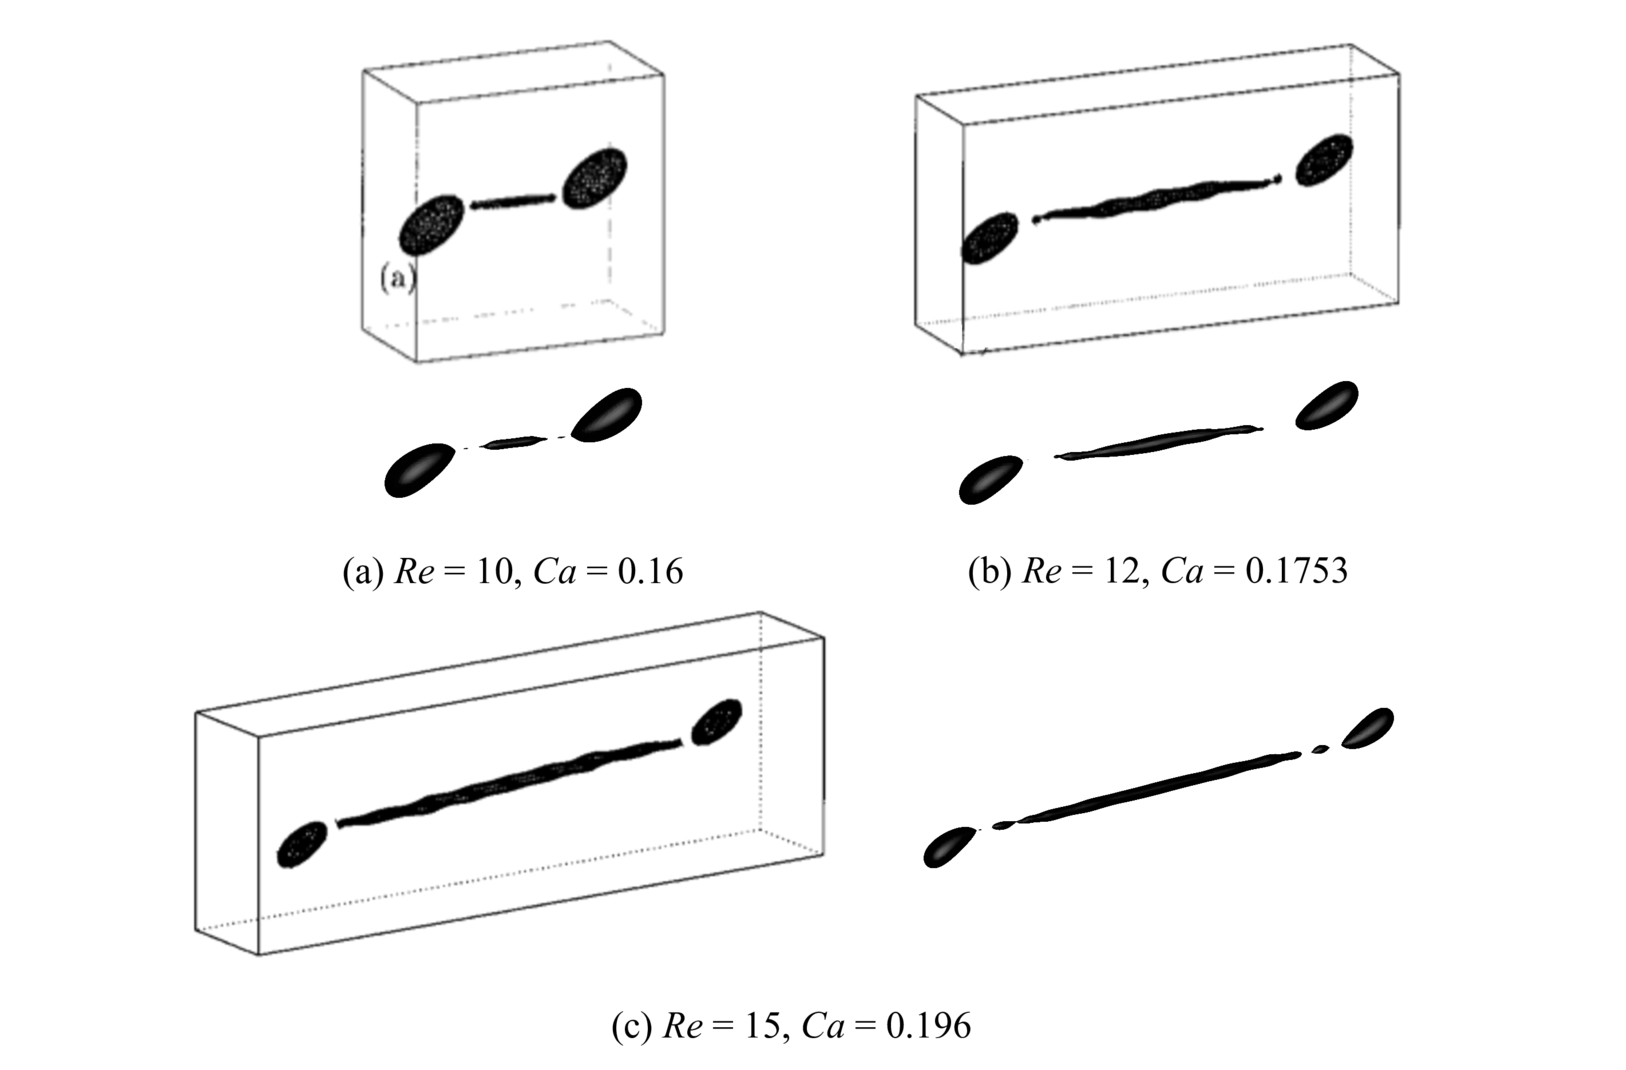
\includegraphics[width=\textwidth]{DropBreakComparison}
  \caption{Comparison with results reported in~\cite{RenCri01-2} (shown in boxes) 
           for drop breakup in shear flow.  (The computational domain
           dimensions $W=4R$ and $H=8R$ were fixed, while $L$ was changed depending 
           on $Re$ and $Ca$ conditions, and the grid size was set to 
           $\Delta x=\Delta y=\Delta z=R/8$.  Reprinted with permission from 
           reference~\cite{RenCri01-2}. Copyright 2001, AIP Publishing). Results
           obtained with our CLSVOF algorithm, corresponding to each case in
           reference~\cite{RenCri01-2}, are shown outside boxes.  The
           CLSVOF method used a two-level AMR computational domain 
           with a level-0 discretization $\Delta x^{\ell=0} = \Delta y^{\ell=0} 
           = \Delta z^{\ell=0} = R/8$ and a level-1 discretization
           $\Delta x^{\ell=1} = \Delta y^{\ell=1} = \Delta z^{\ell=1} = R/16$. 
           The onset of drop breakup is demonstrated for (a) $Re=10$,
           $Ca=0.16$, (b) $Re=12$, $Ca=0.1753$, and (c) $Re=15$, $Ca=0.196$.
           For all three $Re$ and $Ca$ conditions, $\lambda = \eta = 1$.}
  \label{fig:DropBreakComp}
\end{figure}
%

Next, we present a comparison with numerical results for drop breakup reported
in~\cite{RenCri01-2}.  Figure~\ref{fig:DropBreakComp} demonstrates drop breakup
with pinch-off behavior for three $Re$ and $Ca$ conditions and with constant
values of $\lambda = \eta = 1$ for all cases.  The three cases that we consider
correspond to (a) $Re = 10, \, Ca = 0.16$, (b) $Re = 12, \, Ca = 0.1753$, and
(c) $Re = 15, \, Ca = 0.196$, and which are illustrated in
Figures~\ref{fig:DropBreakComp}(a)-(c), respectively.  The results reported
in~\cite{RenCri01-2}, which were obtained with a VOF method, are shown inside
boxes while results obtained with our CLSVOF approach are displayed outside
boxes.  In the computations presented in~\cite{RenCri01-2}, the dimensions
$W=4R$ and $H=8R$ were fixed, while $L$ was changed depending on $Re$ and $Ca$
conditions, and the grid size was set to $\Delta x=\Delta y=\Delta z=R/8$.  To
compare with their results, we performed simulations with the CLSVOF method
over a two-level AMR computational domain of the same dimensions and the same
level-0 discretization: $\Delta x^{\ell=0} = \Delta y^{\ell=0} = \Delta
z^{\ell=0} = R/8$; we set the finer level-1 grid size $\Delta x^{\ell=1} =
\Delta y^{\ell=1} = \Delta z^{\ell=1} = R/16$.  The results shown in
Figure~\ref{fig:DropBreakComp} verify that our numerical approach can reproduce
the same drop breakup behavior presented in~\cite{RenCri01-2}.  Slight
differences between the results can be attributed to the increased resolution
used in our study in the level-1 grid around the elongated drop.  The numerical
validation studies performed in this section demonstrate that our numerical
method is capable of accurately simulating shear-induced drop deformation and
breakup.

\subsection{Consideration of domain and grid sizes}\label{sec:DomGrdSize}
%  -----------------------------------------------------------------------------
The computational domain size used in numerical studies can affect the behavior
of drop deformation and breakup.  Referring to
Figure~\ref{fig:SchemAndGrid}(a), with an appropriately large domain length $L$
and a fixed width $W=4R$, the effect of the height $H$ on drop behavior was
examined in~\cite{LiRenRen00} for Stokes flows and various $Ca$ conditions and
in~\cite{KomShaEskDer14} for $Re=1$ and $Ca=0.27$.  Other related studies
investigated drop breakup sensitivity~\cite{RenCri01-1} and drop deformation
sensitivity~\cite{RenCriLi02} with respect to the entire domain size.
%
\begin{table}[tbh]
\caption{Comparison of the Taylor deformation parameter $De$ for a drop as a function of
         domain size ($Re=0.75$, $Ca=0.3$, $\lambda = \eta = 1$).
         CLSVOF method computations used a two-level AMR computational domain 
         with a level-0 discretization $\Delta x^{\ell=0} = \Delta y^{\ell=0} 
         = \Delta z^{\ell=0} = R/8$ and a level-1 discretization
         $\Delta x^{\ell=1} = \Delta y^{\ell=1} = \Delta z^{\ell=1} = R/16$.}
\label{tab:DomComparison}
%\footnotesize
\center
\begin{tabular}{ c  c  c}
\hline
\hline
System      & Domain size ($\LWH$)         & $De$    \\
System 1    & $8R  \times 4R  \times 8R$   & Breakup \\
System 2    & $12R \times 4R  \times 8R$   & Breakup \\
System 3    & $8R  \times 4R  \times 6R$   & 0.541   \\
System 4    & $8R  \times 6R  \times 6R$   & 0.466   \\
System 5    & $8R  \times 8R  \times 8R$   & 0.460   \\
System 6    & $8R  \times 16R \times 16R$  & 0.460   \\
\hline
\hline
\end{tabular}
\end{table}
%

Here we investigate the drop dynamics sensitivity to domain size around the
critical Reynolds number $Re_{c}=0.75$.  Specifically, we consider domain size
sensitivity for the condition of $Re=0.75$, $Ca=0.3$, and $\lambda = \eta = 1$,
which is a condition used in the comparison studies of the previous section.
As shown in Table~\ref{tab:DeComparison}, the drop breaks up for the condition
of $Re=0.75$ and $Ca=0.3$ with a domain size of $\lwh{8}{4}{8}$.  Results for
domain size sensitivity for six domain systems, all of which use a level-1 grid
size $\Delta x^{\ell=1} = \Delta y^{\ell=1}= \Delta z^{\ell=1} = R/16$, are
tabulated in Table~\ref{tab:DomComparison}. Note that the domain size used in
the comparison study (Table~\ref{tab:DeComparison}) corresponds to System 1.

The results in Table~\ref{tab:DomComparison} suggest that drop deformation is
promoted when we use a domain size with $W=4R$.  In contrast, the drop does not
break up and becomes stable with a deformed shape if we set $L$ large enough
and $W \geq 6R$ and $H \geq 6R$.  Since the value of $De$ for the domain size
$\lwh{8}{6}{6}$ differs by only $1.3\%$ with the value for the domain size of
$\lwh{8}{16}{16}$, in the results that follow we set the width to $W=6R$ and the
height to $H=6R$ to minimize the number of computational grid nodes along those
directions.  To determine the critical Reynolds number $Re_c$ (with $Ca=0.3$),
we consider a domain size of $\lwh{24}{6}{6}$, and we find that the drop
reaches a stable state with deformation parameter $De=0.549$ for $Re=1.0$,
while a value of $Re=1.1$ leads to drop breakup.
% 
\begin{figure}%[h!]
  \centering
  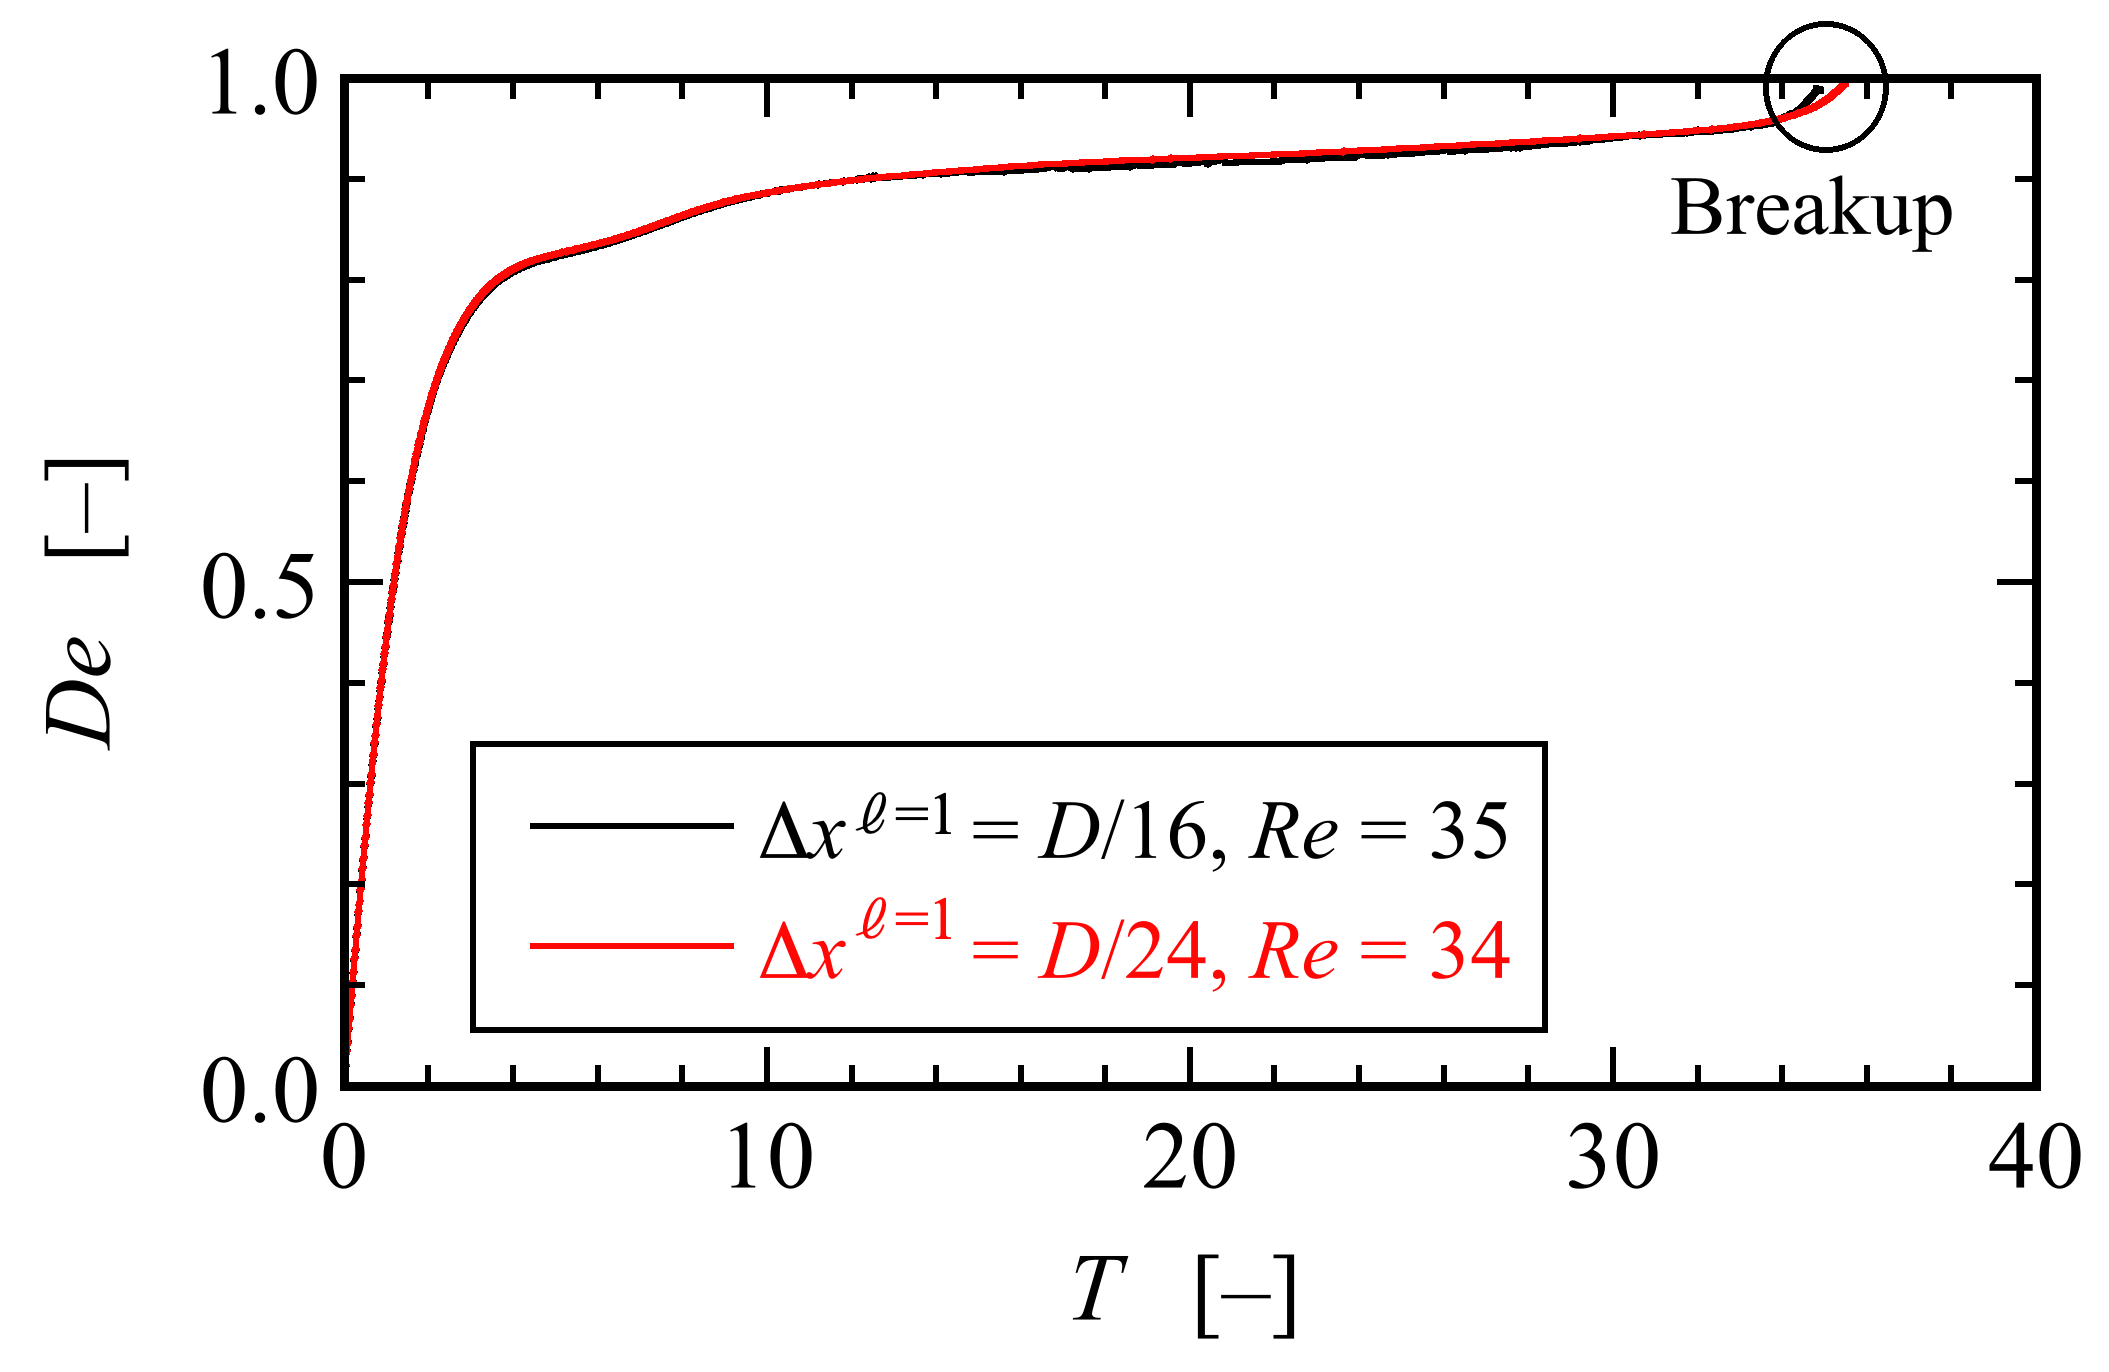
\includegraphics[width=\textwidth]{DeEvolution}
  \caption{Time evolution of the deformation parameter $De$ versus 
   a dimensionless
   time $T = \mathit{\Gamma} t$ for a bubble, obtained 
   with two grid systems at different resolutions. Both systems use a 
   two-level AMR grid with a uniform 
   finest-level grid size $\Delta x^{\ell=1} = \Delta y^{\ell=1} = 
   \Delta z ^{\ell=1}$. The evolution of $De$ using the first system, where
   $\Delta x^{\ell=1} = R/16$, is shown in black and it predicts that 
   bubble breakup occurs at a Reynolds number $Re=35$. 
   Results with the second system, shown in red, use $\Delta x^{\ell=1} 
   = R/24$, and they predict that breakup occurs at $Re=34$.  The capillary
   number corresponding to these results is $Ca=1.0$.
   ($\lambda$ = $\eta$ = 1.0 $\times$ $10^{-3}$)}
  \label{fig:DeEvolution}
\end{figure}
%

The numerical results presented in this and the previous section used a
finest-level grid size set to $\Delta x^{\ell=1}(= \Delta y^{\ell=1}= \Delta
z^{\ell=1})=R/16$. To verify the adequacy of this grid resolution, we present
grid refinement results for a bubble breakup simulation with $Ca=1.0$, which
corresponds to the most deformable and stretchable bubble case considered in
our numerical studies. We use two different grid systems, one with $\Delta
x^{\ell=1}=R/16$ and another with $\Delta x^{\ell=1}=R/24$, to determine
$Re_c$.  Figure~\ref{fig:DeEvolution} shows the time evolution of the
deformation parameter $De$ over time for the two grid systems; the $x$-axis is
a dimensionless time defined by $T=\mathit{\Gamma} t$ and the $y$-axis is $De$.
The results show that bubble breakup occurs at $Re_c = 35$ for the grid system
with $\Delta x^{\ell=1}=R/16$, while the finer computational grid with $\Delta
x^{\ell=1}=R/24$ predicts a critical value of $Re_c = 34$.  Note that although
the time evolution of $De$ for the two grid systems is consistent for both
resolutions (the predicted critical Reynolds numbers differ by $\sim 3\%$), the
computational time using the grid system with $\Delta x^{\ell=1}=R/24$ was more
than 6 times longer than the one based on the coarser system with $\Delta
x^{\ell=1}=R/16$.  We remark that in our search for $Re_c$, we considered a
wide range of values of $Ca$ and we found it necessary to use a large $L$
($\sim 24R$) since for certain shear flows the bubble can stretch significantly
without breaking up.  Nevertheless, for the conditions presented in this
section, the results indicate that our numerical approach, even with a
finest-level resolution set to $\Delta x^{\ell=1}=R/16$, is capable of
accurately reproducing bubble deformation and breakup without sacrificing any
essential dynamical features.


%  -----------------------------------------------------------------------------
\section{Results and Discussion}
%  -----------------------------------------------------------------------------

\subsection{Drop deformation and breakup}\label{sec:DropBreak}
%  -----------------------------------------------------------------------------
% 
\begin{figure}%[h!]
  \centering
  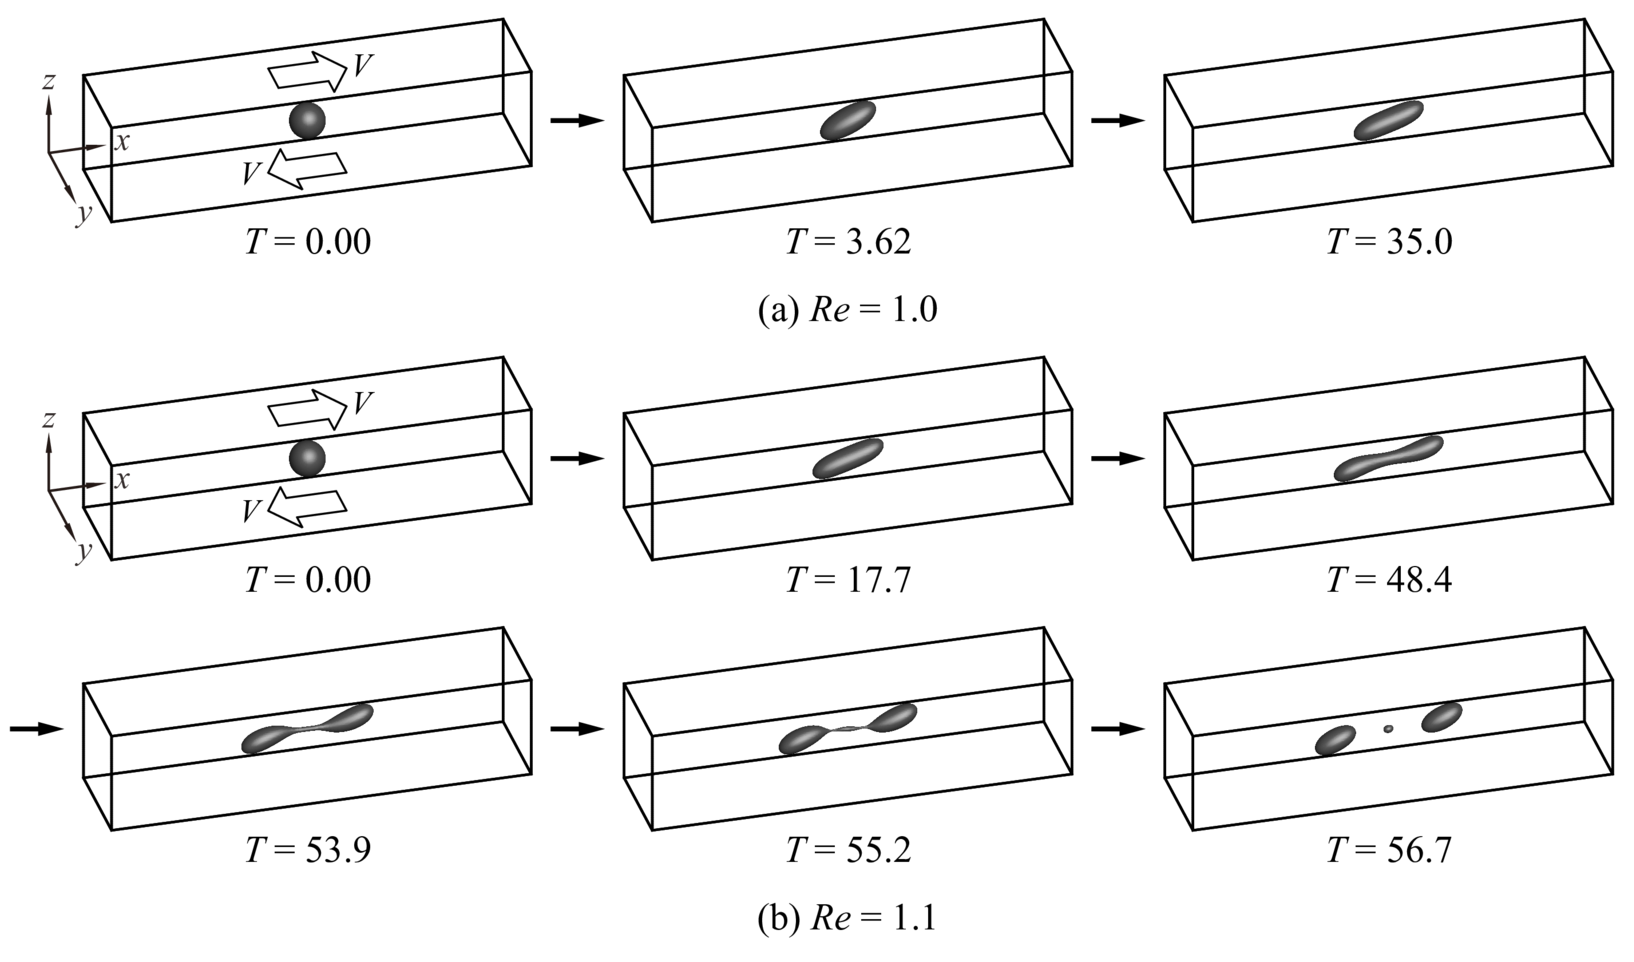
\includegraphics[width=\textwidth]{DropBreakEvol}
  \caption{Time evolution of drop deformation and breakup in shear flow at the
           condition of $Ca=0.3$ with (a) $Re=1.0$ and (b) $Re=1.1$.  The
	   ``drop'' critical Reynolds number corresponding to $Ca=0.3$ is
	   $1.0<Re_{c}<1.1$.
	   ($\lambda$ = $\eta$ = 1.0)}
  \label{fig:DropBreak}
\end{figure}
%
To illustrate the differences in deformation and breakup between a drop and a
bubble around critical conditions, we first present numerical results for drop
deformation.  The time evolution of drop deformation and breakup in simple
linear shear flow for two conditions is shown in Figure~\ref{fig:DropBreak};
the first case, shown in Figure~\ref{fig:DropBreak}(a), uses $Ca=0.3$ and
$Re=1.0$, while the second case, depicted in Figure~\ref{fig:DropBreak}(a),
uses $Ca=0.3$ and $Re=1.1$.  Using a domain size of $\lwh{24}{6}{6}$, in the
case with $Re=1.0$, the drop gradually deforms and finally attains a stable
deformed state with $De$= 0.549.  Over the same domain, for the case with
$Re=1.1$, the ``mother'' drop elongates over time and the volume at the ends of
the deforming drop expands; that is, both ends of the drop become bulb-shaped.
As time progresses, particularly over the time interval $48.4 \leq T \leq
55.2$, a thread-bridge forms between the bulbous ends and the thread-bridge
becomes thinner.  Finally, at around the dimensionless time $T\sim 56.7$, the
mother drop breaks up, forming two ``daughter'' drops through the pinch off;
one satellite drop is also generated between the pinched off daughter drops.


\subsection{Bubble deformation and breakup}
%  -----------------------------------------------------------------------------
% 
\begin{figure}%[h!]
  \centering
  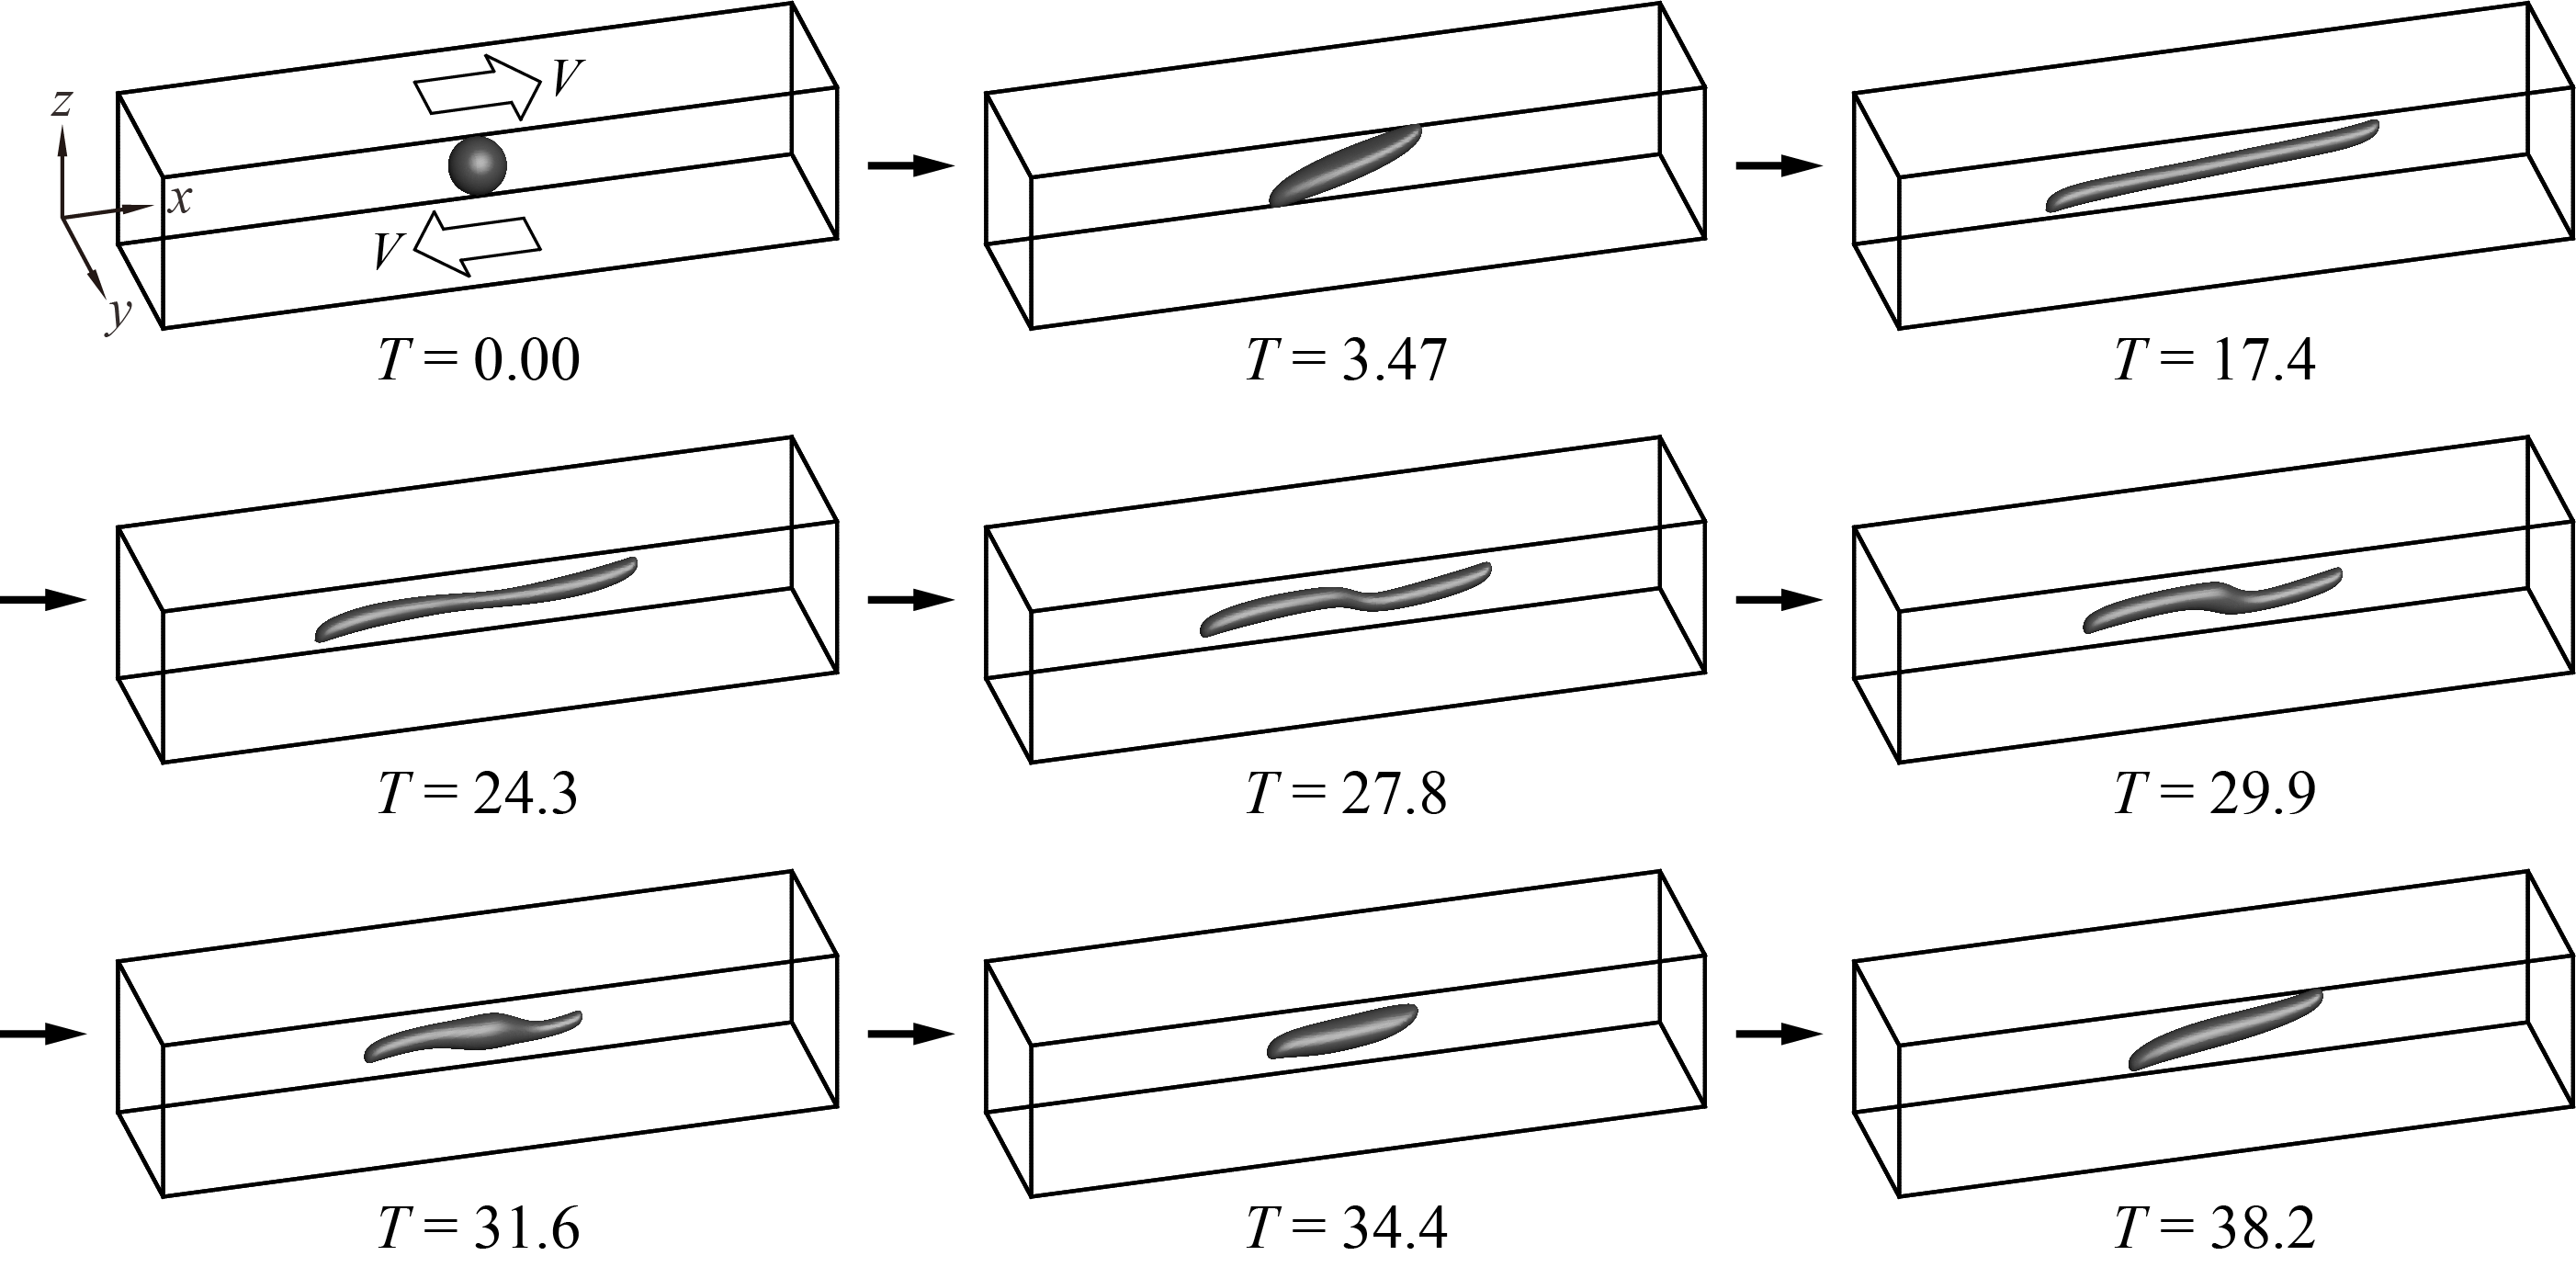
\includegraphics[width=\textwidth]{BubbleBreakCa0p3Re92}
  \caption{Time evolution of bubble deformation in shear flow at the
           condition of $Ca=0.3$ and $Re=92$.  
	   The ``bubble'' 
	   critical Reynolds number corresponding to $Ca=0.3$ is
	   $92<Re_{c}<93$.  In contrast to the drop deformation case,
           when $Re$ is slightly below $Re_{c}$
           (See Figure \ref{fig:DropBreak} $Re=1.0$ for the drop case), 
           the bubble shape will
           not reach a steady shape, instead the bubble shape alternates
           between the shapes ``slightly stretched'' ($T=3.47$),
           fully stretched and ``doglegged'' ($T=27.8$) and ``almost''
           back to the original ``slightly stretched'' case 
           ($T=34.4$). 
           ($\lambda$ = $\eta$ = 1.0 $\times$ $10^{-3}$) 
	   }
  \label{fig:BubbleBreakCa0p3Re92}
\end{figure}
%
\begin{figure}%[h!]
  \centering
  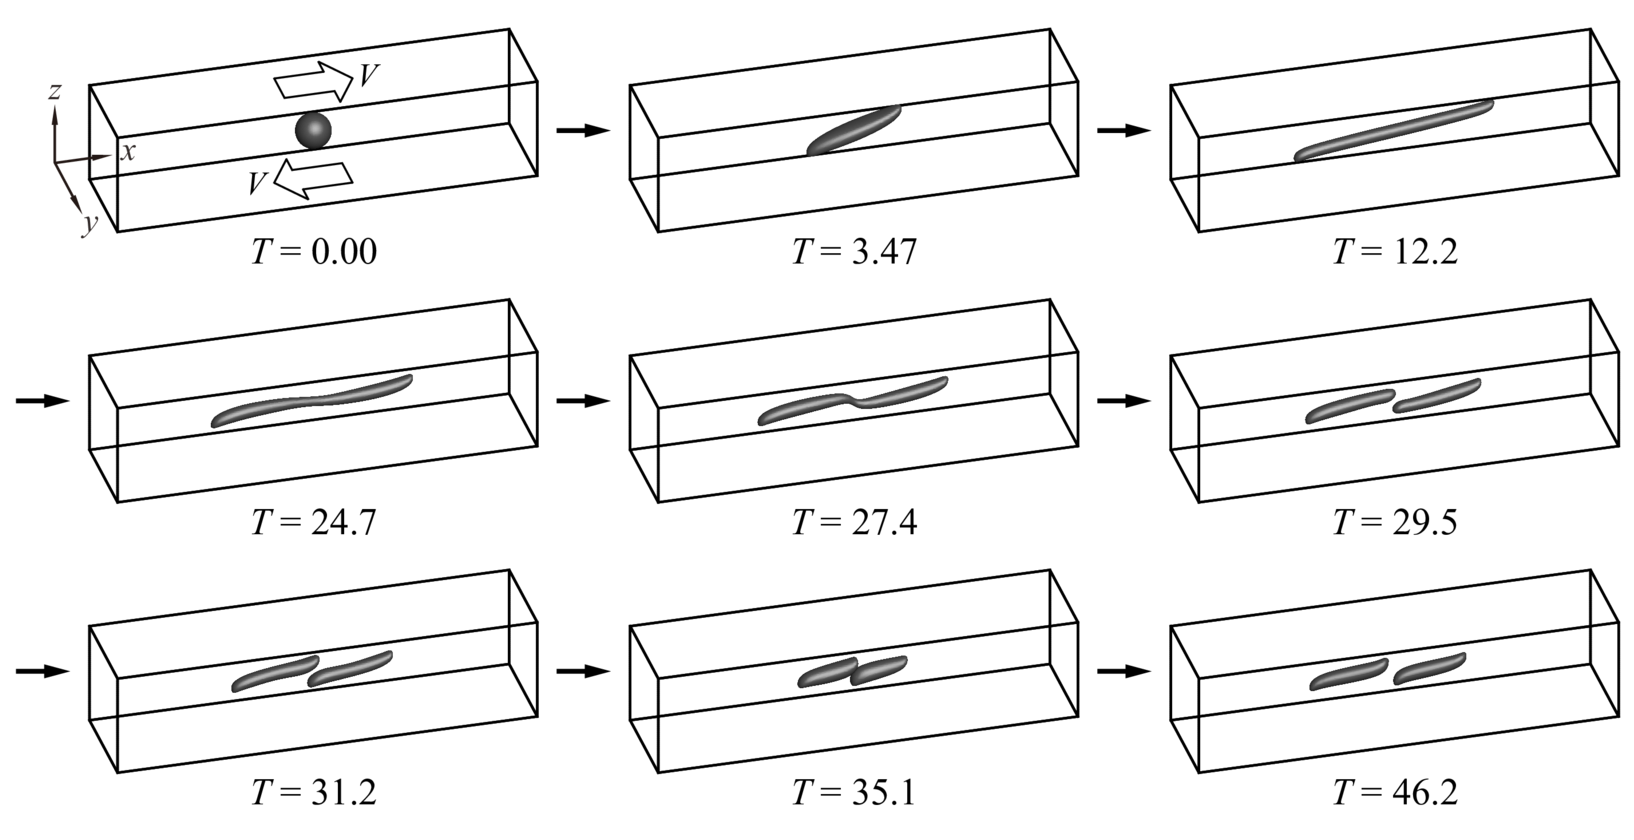
\includegraphics[width=\textwidth]{BubbleBreakCa0p3Re93}
  \caption{Time evolution of bubble deformation in shear flow at the
           condition of $Ca=0.3$ and $Re=93$.
	   The ``bubble'' 
	   critical Reynolds number corresponding to $Ca=0.3$ is
	   $92<Re_{c}<93$.
           ($\lambda$ = $\eta$ = 1.0 $\times$ $10^{-3}$) 
	   }
  \label{fig:BubbleBreakCa0p3Re93}
\end{figure}
%
Next we present numerical results that illustrate the conditions that lead to
bubble deformation without breakup as well as conditions where the bubble
deforms and ultimately breaks up.  The time evolution of shear-induced bubble
deformation without breakup at the condition of $Ca=0.3$ and $Re=92$ is
depicted in Figure~\ref{fig:BubbleBreakCa0p3Re92} and the bubble breakup
process with flow condition of $Ca=0.3$ and $Re=93$ is illustrated in
Figure~\ref{fig:BubbleBreakCa0p3Re93}.  The results indicate that the critical
Reynolds number is approximately $Re_c = 93$ (with $Ca=0.3$).  A comparison
with the drop breakup dynamics presented in Section~\ref{sec:DropBreak} and the
corresponding processes for bubble deformation and breakup exhibit very
distinct features.  First, we note that a relatively large shear force
magnitude is required for bubble breakup 
($\lambda$ = $\eta$ = 1.0 $\times$ $10^{-3}$) 
compared with the case of the drop ($\lambda$ = $\eta$ = 1). Then,
for the same value of $Ca=0.3$, the critical Reynolds number for the bubble is
around 85 times larger than that for the drop.  Focusing on the bubble dynamics
with no-breakup (Figure~\ref{fig:BubbleBreakCa0p3Re92}), the results show that
the bubble is largely elongated in the $x$-direction at the early stages ($T
\leq 24.3$) of bubble deformation, but the bubble does not develop the
bulb-like shape (large volume areas) at both ends present in the drop
deformation process.  It is also evident that the ends of the deforming bubble
develop cusped shapes under the influence of the strong shear flow.  A
noteworthy feature for the non-breaking bubble is that it does not settle into
a deformed stable state as in the case of drop deformation presented in
Figure~\ref{fig:DropBreak}(a).  After an initial elongation process, the bubble
enters a shrinking phase ($T = 27.8$) where the doglegged shape formed at the
center of the bubble returns to a smaller deformed shape ($T = 34.4$) that is
similar to its earlier shape ($T=3.47$).  However, when we compare the early
deformed bubble shape at $T = 3.47$ with the shape at $T = 34.4$, it is clear
that the shapes are not identical.  Following the shrinking phase, the bubble
begins to stretch again ($T = 38.2$) and the bubble oscillates between its
elongated shape and shortened geometry.  

%
\begin{figure}%[h!]
  \centering
  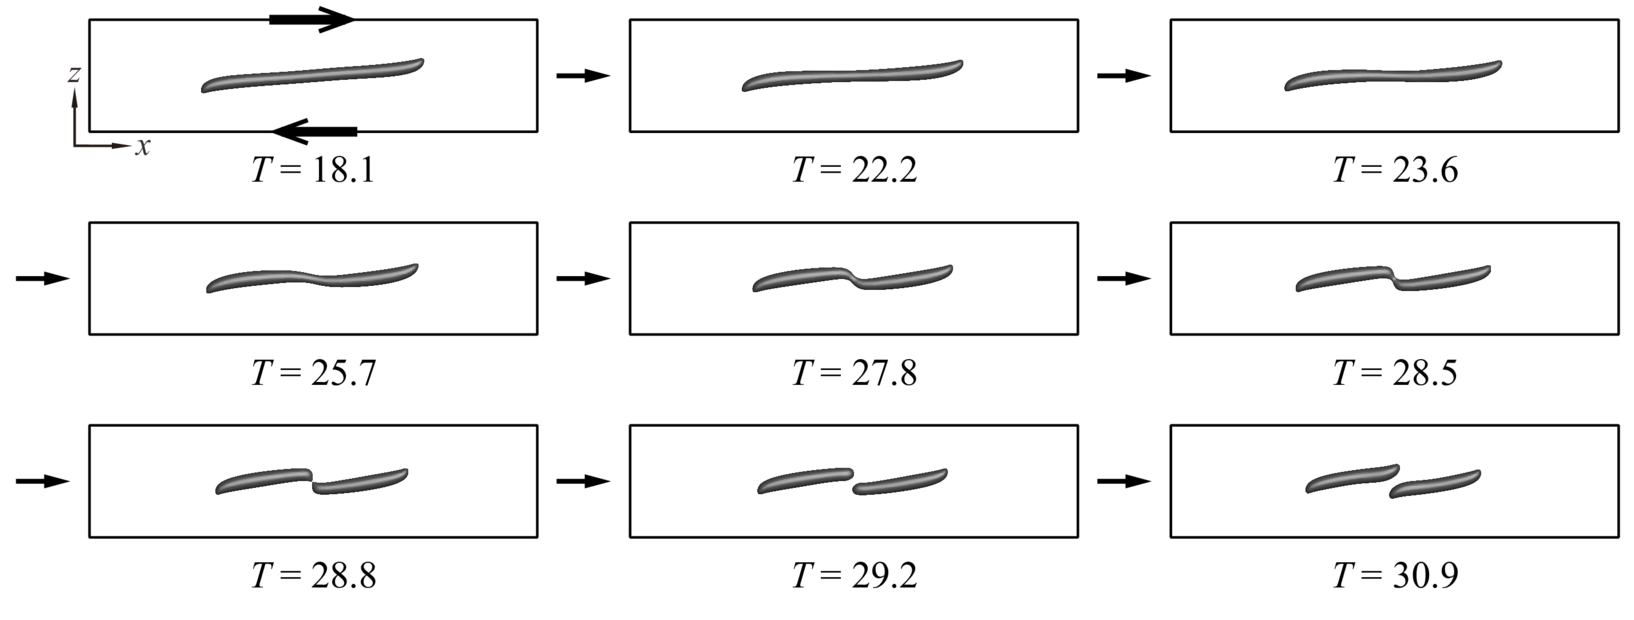
\includegraphics[width=\textwidth]{BubBreakCa0p3Re93Detail}
  \caption{Detail of bubble breakup process in shear flow at the condition
           of $Ca=0.3$ and $Re=93$.
	   The ``bubble'' 
	   critical Reynolds number corresponding to $Ca=0.3$ is
	   $92<Re_{c}<93$.
           ($\lambda$ = $\eta$ = 1.0 $\times$ $10^{-3}$) 
	   }
  \label{fig:BubBreakCa0p3Re93Detail}
\end{figure}
%
For the case of bubble breakup (Figure~\ref{fig:BubbleBreakCa0p3Re93}), we
observe that the deformation process is the almost same as the no-breakup case
until the doglegged shape is formed at $T \sim 27.4$. The bubble finally breaks
during the time interval $27.7 \leq T \leq 29.5$.  For a closer examination of
the bubble breakup process, a detailed panel of cross-sectional slices in the
$xz$-plane through the bubble shape center is presented in
Figure~\ref{fig:BubBreakCa0p3Re93Detail}.  The images displayed in
Figure~\ref{fig:BubBreakCa0p3Re93Detail}, which are taken at shorter time
intervals than those shown in Fig.~\ref{fig:BubbleBreakCa0p3Re93}, reveal that
the bubble breaks up into two daughter bubbles due to the pinch off at the
thread-bridge part of the doglegged shape during the shrinking process ($T =
28.5 \sim 28.8$).  After breaking up, the two daughter bubbles migrate to the
center: the left daughter bubble moves toward the right-side of the domain and
the right daughter bubble moves to the left side (see results for $T = 29.5
\sim 35.1$ in Figure~\ref{fig:BubbleBreakCa0p3Re93} and for $T = 28.8 \sim
30.9$ in Figure~\ref{fig:BubBreakCa0p3Re93Detail}).  The two daughter bubbles
then momentarily congregate near the domain center ($T = 35.1$ in
Figure~\ref{fig:BubbleBreakCa0p3Re93}), before they slowly start to separate:
the left daughter bubble moves to the left and the right daughter bubble moves
to the right ($T = 46.2$ in Figure~\ref{fig:BubbleBreakCa0p3Re93}).  The
results clearly demonstrate that the bubble breakup process is markedly
different from the analogous drop breakup process. 


\subsection{Velocity field outside and inside the breaking bubble}
%  -----------------------------------------------------------------------------
%
\begin{figure}%[h!]
  \centering
  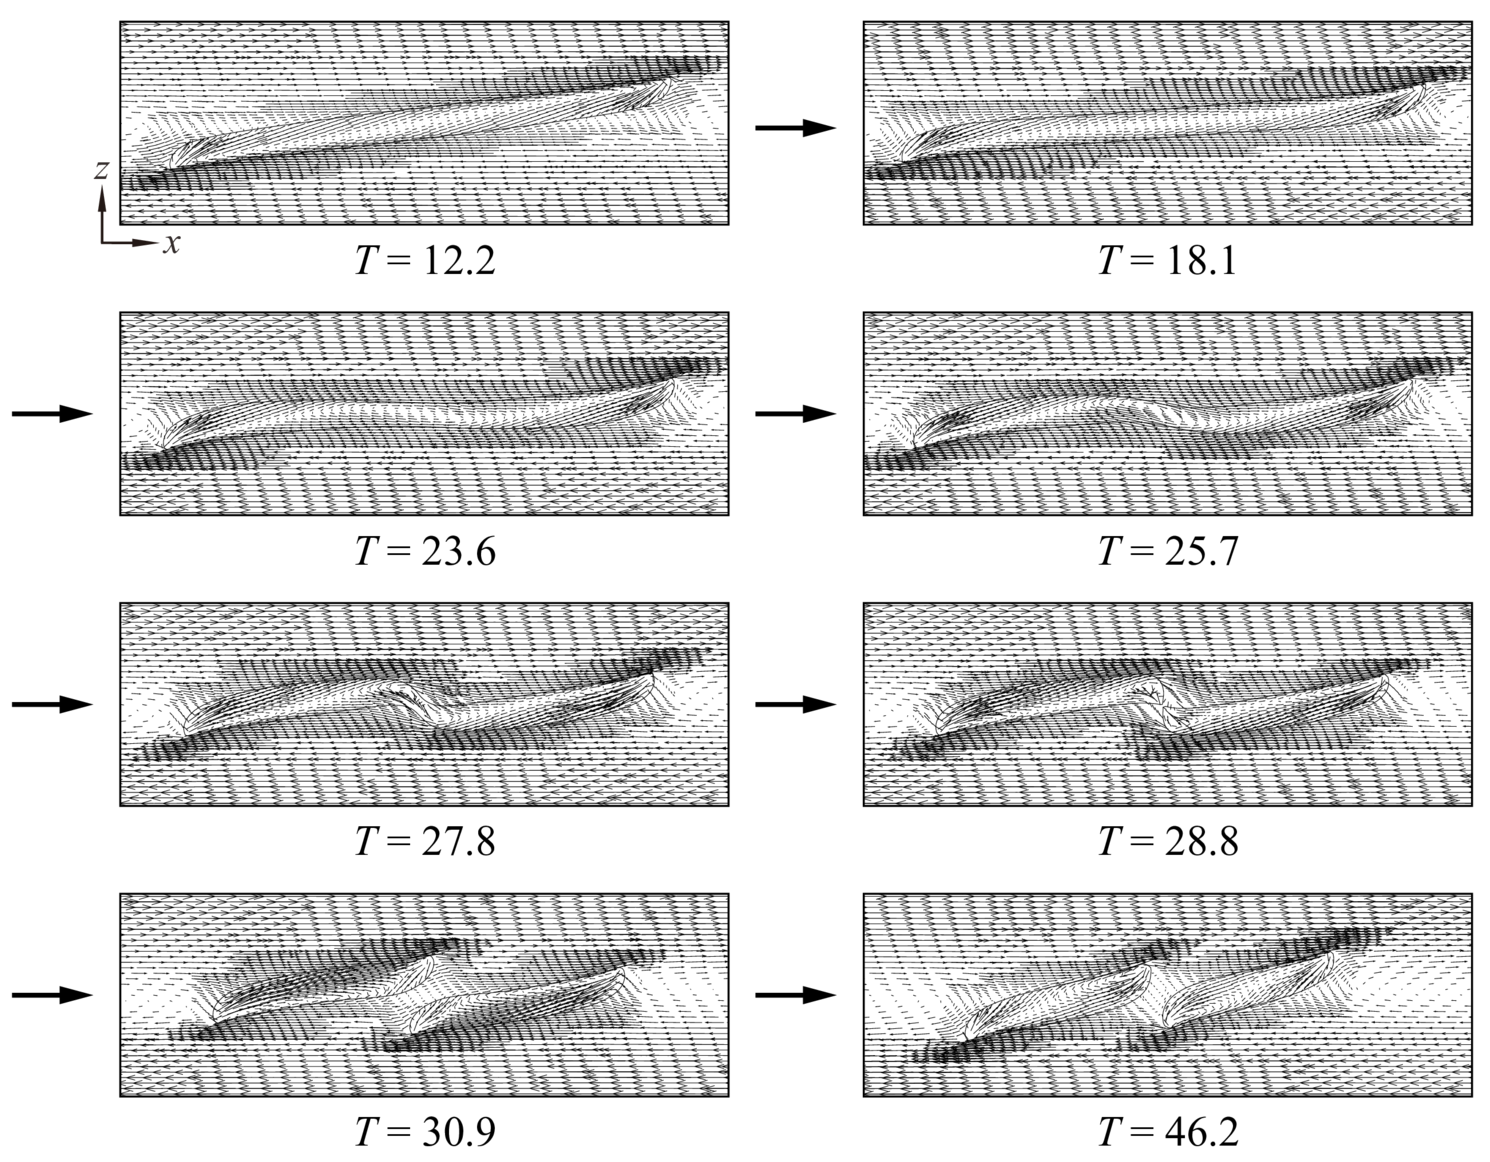
\includegraphics[width=\textwidth]{BubbleFieldCa0p3Re93}
  \caption{Fluid velocity field outside and inside the breaking bubble in
           shear flow at the condition $Ca=0.3$ and $Re=93$.
	   The ``bubble'' 
	   critical Reynolds number corresponding to $Ca=0.3$ is
	   $92<Re_{c}<93$.
           ($\lambda$ = $\eta$ = 1.0 $\times$ $10^{-3}$) 
	   }
  \label{fig:BubbleFieldCa0p3Re93}
\end{figure}
%
In this section, we consider the fluid flow velocity field outside and inside
the bubble during the shear-induced breakup process.
Figure~\ref{fig:BubbleFieldCa0p3Re93} shows the velocity fields outside and
inside the bubble at cross-sectional slices in the $xz$-plane for a flow
condition of $Ca = 0.3$ and $Re = 93$.  Regions around the bubble where there
is a higher density of velocity vectors correspond to the level-1 grid portion
of the AMR structure.  The simulation results show that the velocity field
inside the bubble is particularly distinct from the surrounding flow field in
the exterior of the bubble.  The cross-sections at $T=12.2$ and $T=18.1$, taken
during the elongation phase, show how shear forces at the lower and upper
halves of the bubble act along the bottom and top surfaces, respectively, to
deform the interface.  Near the left and right edges of the bubble, inward
interior flows (that point toward the bubble center) begin to develop.  Strong
shearing forces in the exterior near the bottom-left-end and top-right-end of
the bubble interact with the interior flow field through the boundary to create
cusped shapes at the bottom-left and top-right ends of the bubble while the
interface is laterally elongated in the $x$-direction.  During the shrinking
process, which occurs for $23.6 \leq T \leq 27.8$, inward flows within the
bubble extend over a wider region and are no longer localized near the bubble
edges.  Then, we observe that circulating flows form at the thread-bridge part
of the doglegged bubble shape over the time interval $[25.7, 27.8]$.  During
the breakup process ($T \sim 28.8$), higher-intensity inward flows are formed
inside the bubble, near the pinch off region, that are naturally larger than
the surrounding interior flows and which are inextricably associated with the
bubble migration illustrated in Figs.~\ref{fig:BubbleBreakCa0p3Re93}
and~\ref{fig:BubBreakCa0p3Re93Detail}.  As time proceeds further ($T =  46.2$),
distinct inward flows are formed inside the daughter bubbles; the bubbles then
begin their migration toward the side walls.  Considering the left daughter
bubble, for example, we see that the mechanism responsible for this movement
results from larger shear forces acting on the bottom-left end than those in
the top-left end.


\subsection{Effect of surface tension on bubble deformation and breakup}
%  -----------------------------------------------------------------------------
%
\begin{figure}%[h!]
  \centering
  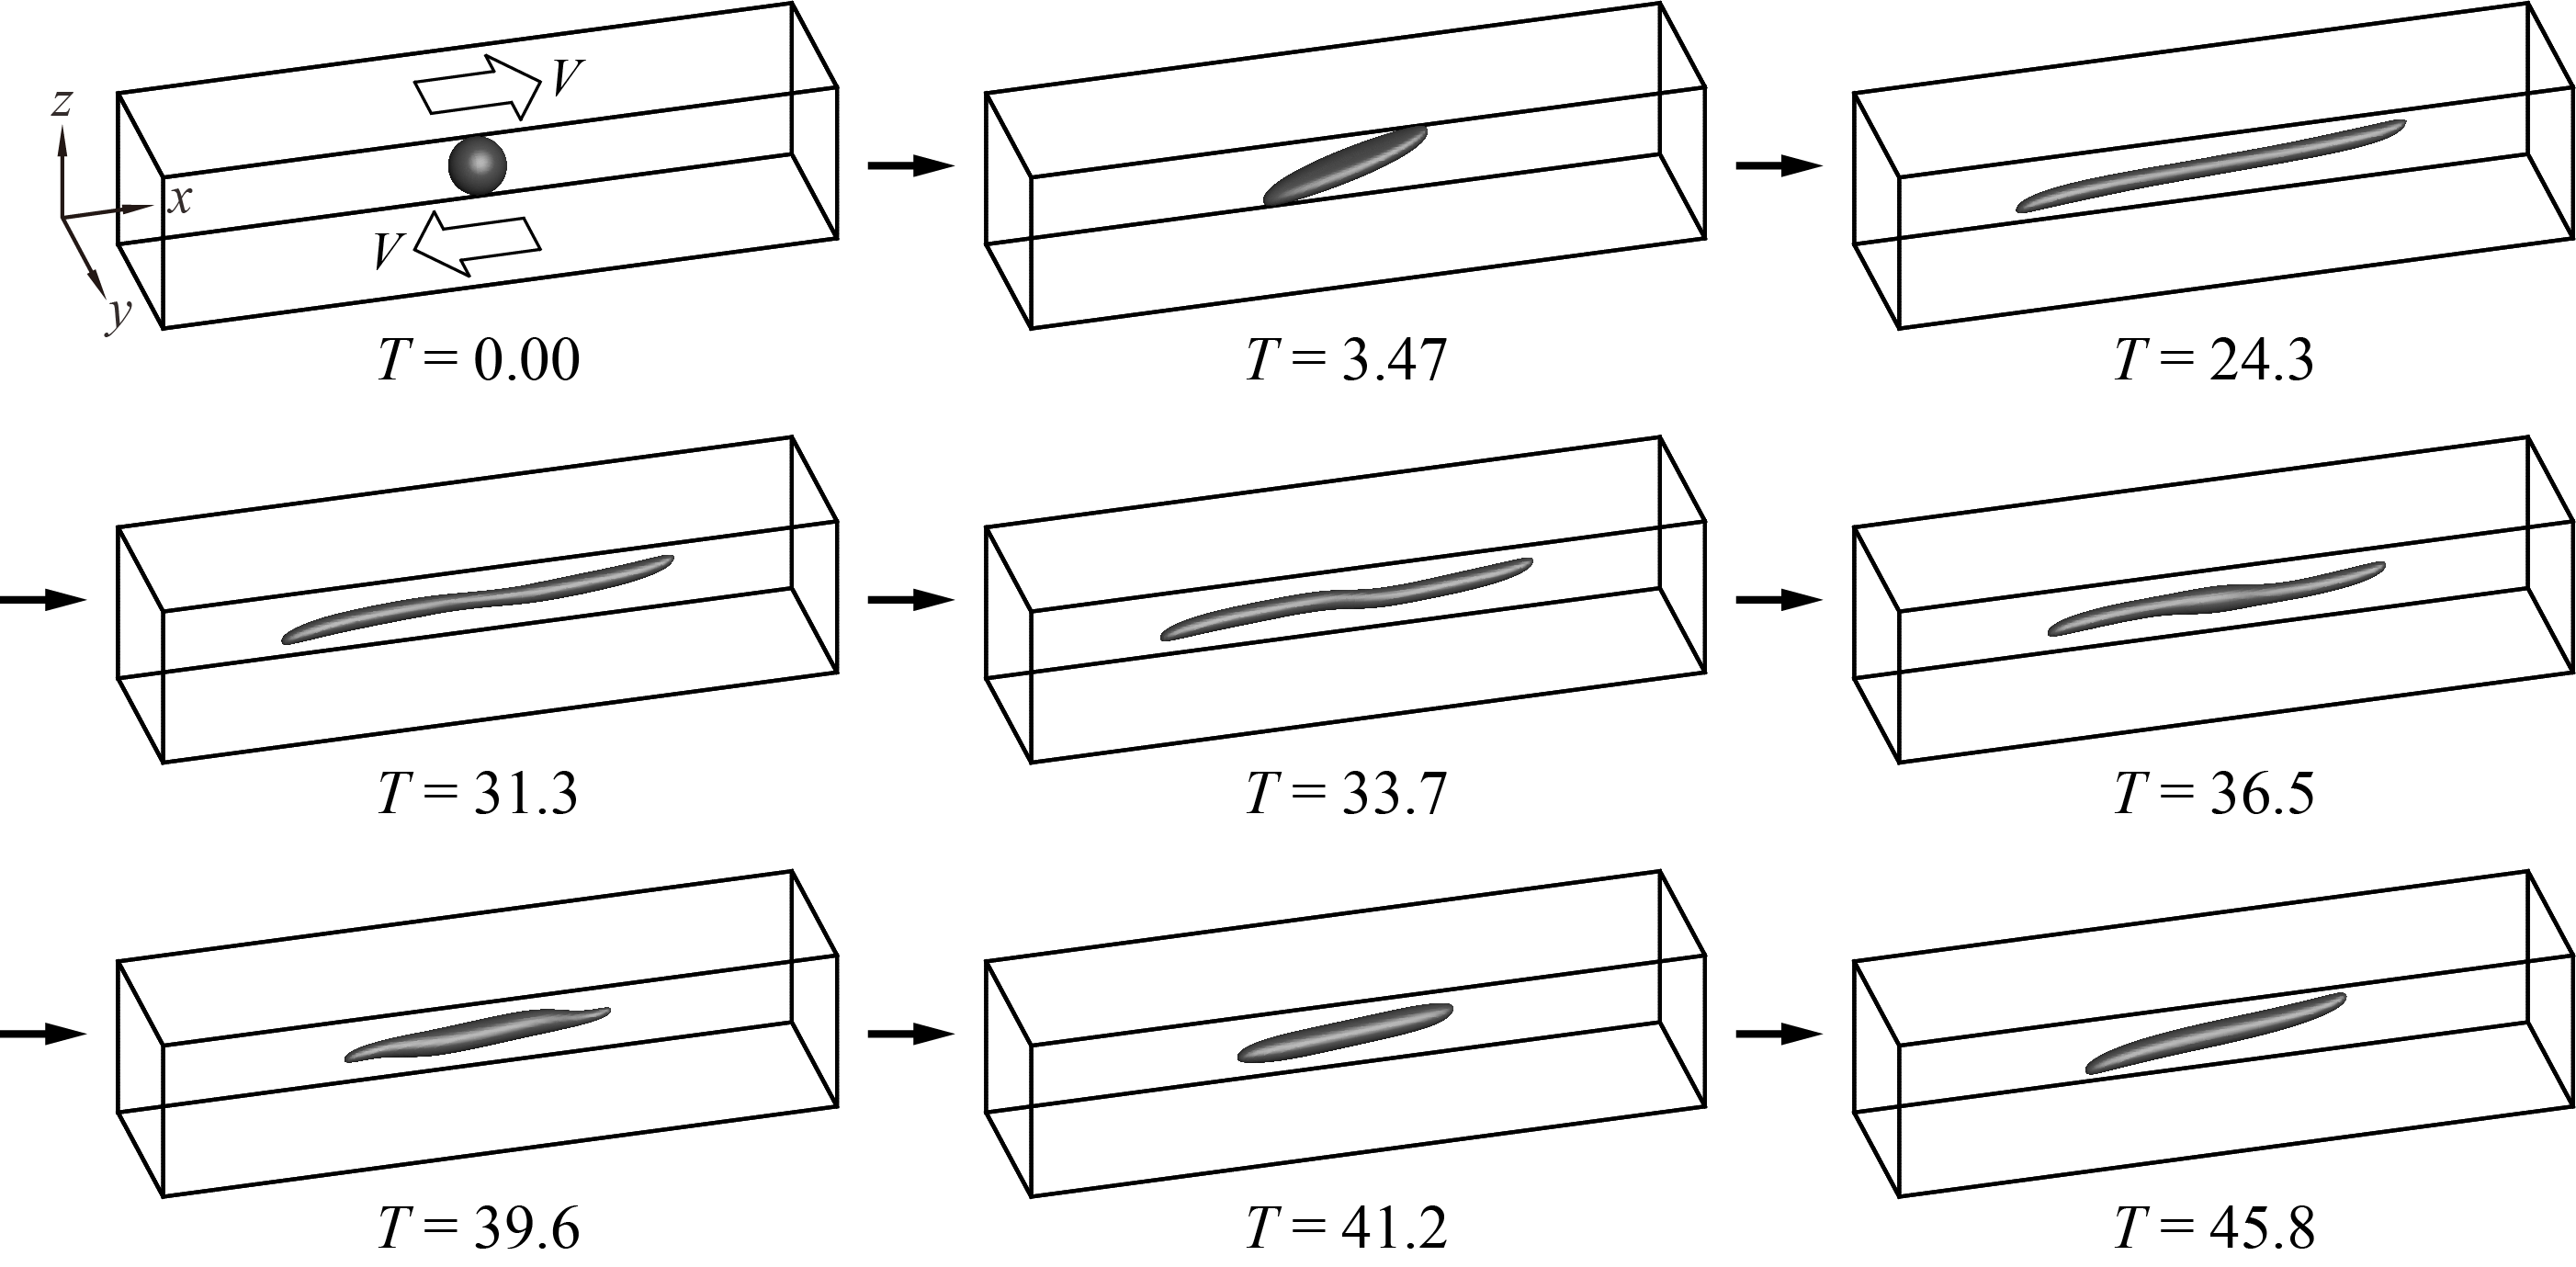
\includegraphics[width=\textwidth]{BubbleDeformCa0p8Re42}
  \caption{Time evolution of bubble deformation in shear flow at the 
           condition of $Ca=0.8$ and $Re=42$.
	   The ``bubble'' 
	   critical Reynolds number corresponding to $Ca=0.8$ is
	   $42<Re_{c}<43$.
           ($\lambda$ = $\eta$ = 1.0 $\times$ $10^{-3}$) 
	   }
  \label{fig:BubDefCa0p8Re42}
\end{figure}
%
\begin{figure}%[h!]
  \centering
  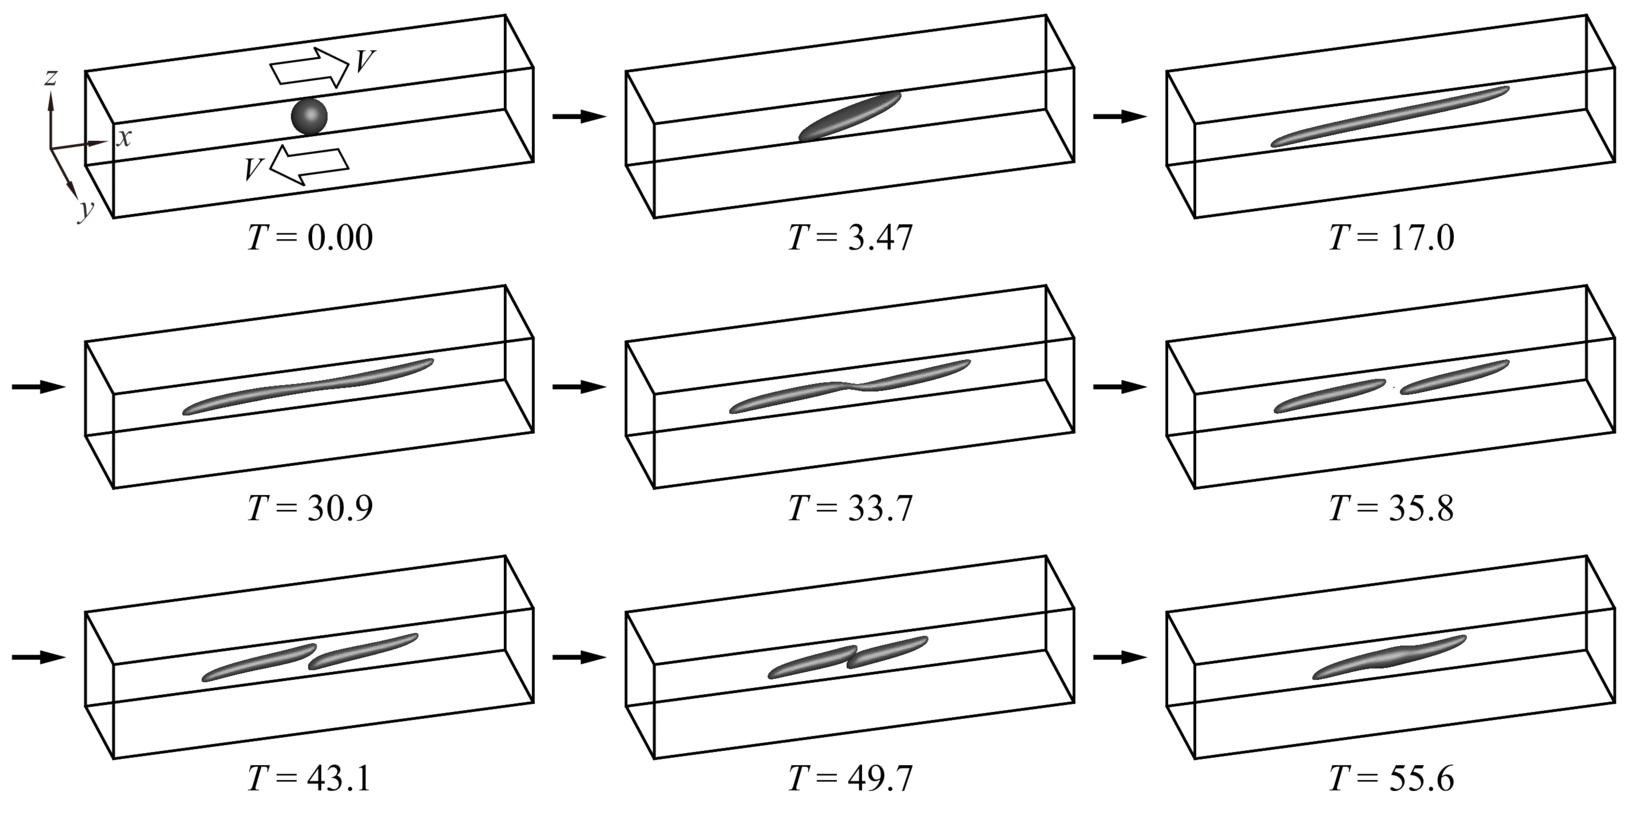
\includegraphics[width=\textwidth]{BubbleBreakCa0p8Re43}
  \caption{Time evolution of bubble deformation in shear flow at the 
           condition of $Ca=0.8$ and $Re=43$.
	   The ``bubble'' 
	   critical Reynolds number corresponding to $Ca=0.8$ is
	   $42<Re_{c}<43$.
           ($\lambda$ = $\eta$ = 1.0 $\times$ $10^{-3}$) 
	   }
  \label{fig:BubBrkCa0p8Re43}
\end{figure}
%
%It means that the effect of the surface tension for the condition of $Ca = 0.8$
%is smaller than that for the condition of $Ca = 0.3$.
%
In previous sections, we considered numerical simulations of bubble deformation
and breakup with a Capillary number $Ca = 0.3$.  Here, we examine similar
bubble dynamics with $Ca = 0.8$ and we also investigate the effect of
interfacial tension on bubble deformation and breakup.  Using $Ca=0.8$ for both
cases, Figures~\ref{fig:BubDefCa0p8Re42} and~\ref{fig:BubBrkCa0p8Re43} present
the time evolution of shear-induced bubble deformation and breakup with $Re=42$
and $Re=43$, respectively.  We note that the bubble critical Reynolds number is
around $Re_{c} \approx 43$, whereas $Re_{c} \approx 0$ for the corresponding
case of the drop with 
$\lambda$ = $\eta$ = 1 (see e.g.~\cite{LiRenRen00}).
Note that $Re_{c}$ for $Ca = 0.8$ is smaller than that for the condition of $Ca
= 0.3$ since the bubble at $Ca = 0.8$ is more elastic due to the weaker effect
of surface tension in this case.  The results shown in
Figs.~\ref{fig:BubDefCa0p8Re42} and~\ref{fig:BubBrkCa0p8Re43} indicate that the
bubble deformation and breakup process for the condition of $Ca = 0.8$ is
analogous to that for $Ca = 0.3$.  For the case of bubble deformation without
breakup (Fig.~\ref{fig:BubDefCa0p8Re42}), the bubble initially assumes a long
elongated shape along the $x$-direction at around $T=24.3$. The bubble then
enters a compression stage over the time interval $[31.3,41.2]$ and
subsequently starts to elongate again at $T = 45.8$.  On the other hand, for
the case of bubble breakup (Fig.~\ref{fig:BubBrkCa0p8Re43}), an initial
elongation phase is followed by a doglegged shape formation at $T=33.7$.  After
that, the bubble ruptures from the thread-bridge part of the doglegged shape
and two daughter bubbles are produced ($T = 35.8$).  The two daughter bubbles
formed after breakup move to the central area ($T = 49.7$) as in the case of
$Ca = 0.8$ and $Re = 93$, but the two bubbles eventually coalesce in a region
approximately centered in the computational domain ($T = 55.6$).  We note that
in a real experimental setting, bubbles may coalesce after breaking up due to
slight deviations of flow conditions and states.  Although the process of
bubble deformation and breakup for flow conditions with $Ca = 0.3$ and $Ca =
0.8$ are similar, a pronounced difference is that the bubble for $Ca = 0.8$ is
more elongated and slender than that for $Ca = 0.3$ due to the smaller effect
of surface tension for $Ca = 0.8$.

Table~\ref{tab:CaRecComparison} 
lists, for representative $Ca$ values,
the corresponding critical Reynolds number, $Re_{c}$, for shear-induced 
bubble breakup for a variety of flow
conditions.  The results indicate that sufficiently large shear forces are
required for bubble breakup even for large Capillary numbers. The combined
effects of very small density and viscosity ratios 
($\lambda$ = $\eta$ = 1.0 $\times$ $10^{-3}$) 
act synergistically in deformation and breakup processes.
We conducted a linear least squares best fit analysis (linear vs. 
power law vs. exponential models) of the data that we 
list in Table~\ref{tab:CaRecComparison} and have found that the following
exponential model is the best fit:
%  Re = \frac{\rho_{b}UR}{\mu_{b}}, \quad
%  Ca = \frac{\mu_{b}U}{\sigma}, \quad
\begin{eqnarray}
Re_{c}=138.3 e^{-1.41 (Ca)} \label{bestfit}
\end{eqnarray}
(\ref{bestfit}) was derived from the linear least squares best fit
of the log of $Re_{c}$:
\begin{eqnarray}
	\log(Re_{c})=4.9-1.41 (Ca)  \label{bestfitraw}
\end{eqnarray}
%% variance for X^T X c = b
%% (S/(n-m)) (X^T X)^{-1}
%% standard deviation: sqrt(4.2E-3)=.07 and sqrt(8.4E-3)=0.09
The predicted variances for the parameters 
``$4.9$'' and ``$-1.41$'' which appear in (\ref{bestfitraw}) are
$4.2E-3$ and $8.4E-3$ respectively.  In other words, even with just
four data points, we have computed a reasonable best fit curve.

In Figure~\ref{fig:CaRecFit} we plot our best fit curve and make the
hypothesis that a given $(Ca,Re)$ pair will result in bubble break up
if the point $(Ca,Re)$ is above the critical curve, 
$0.3<Ca<1$, and the initial/boundary conditions are given
by (\ref{IC_BC}).

%
\begin{table}[tbh]
\caption{Shear-induced bubble breakup for various flow 
	conditions described in terms
        of column pairs of critical Reynolds numbers and 
	corresponding Capillary numbers.
        ($\lambda$ = $\eta$ = 1.0 $\times$ $10^{-3}$) 
	}
\label{tab:CaRecComparison}
\footnotesize
\center
\begin{tabular}{ c  c  c  c  c }
\hline
\hline
Capillary number $Ca$            & 0.3  & 0.5  & 0.8  & 1.0  \\
Critical Reynolds number $Re_c$  & 93   & 67   & 43   & 35   \\
\hline
\hline
\end{tabular}
\end{table}

%% variance for X^T X c = b
%% (S/(n-m)) (X^T X)^{-1}
\begin{figure}%[h!]
  \centering
  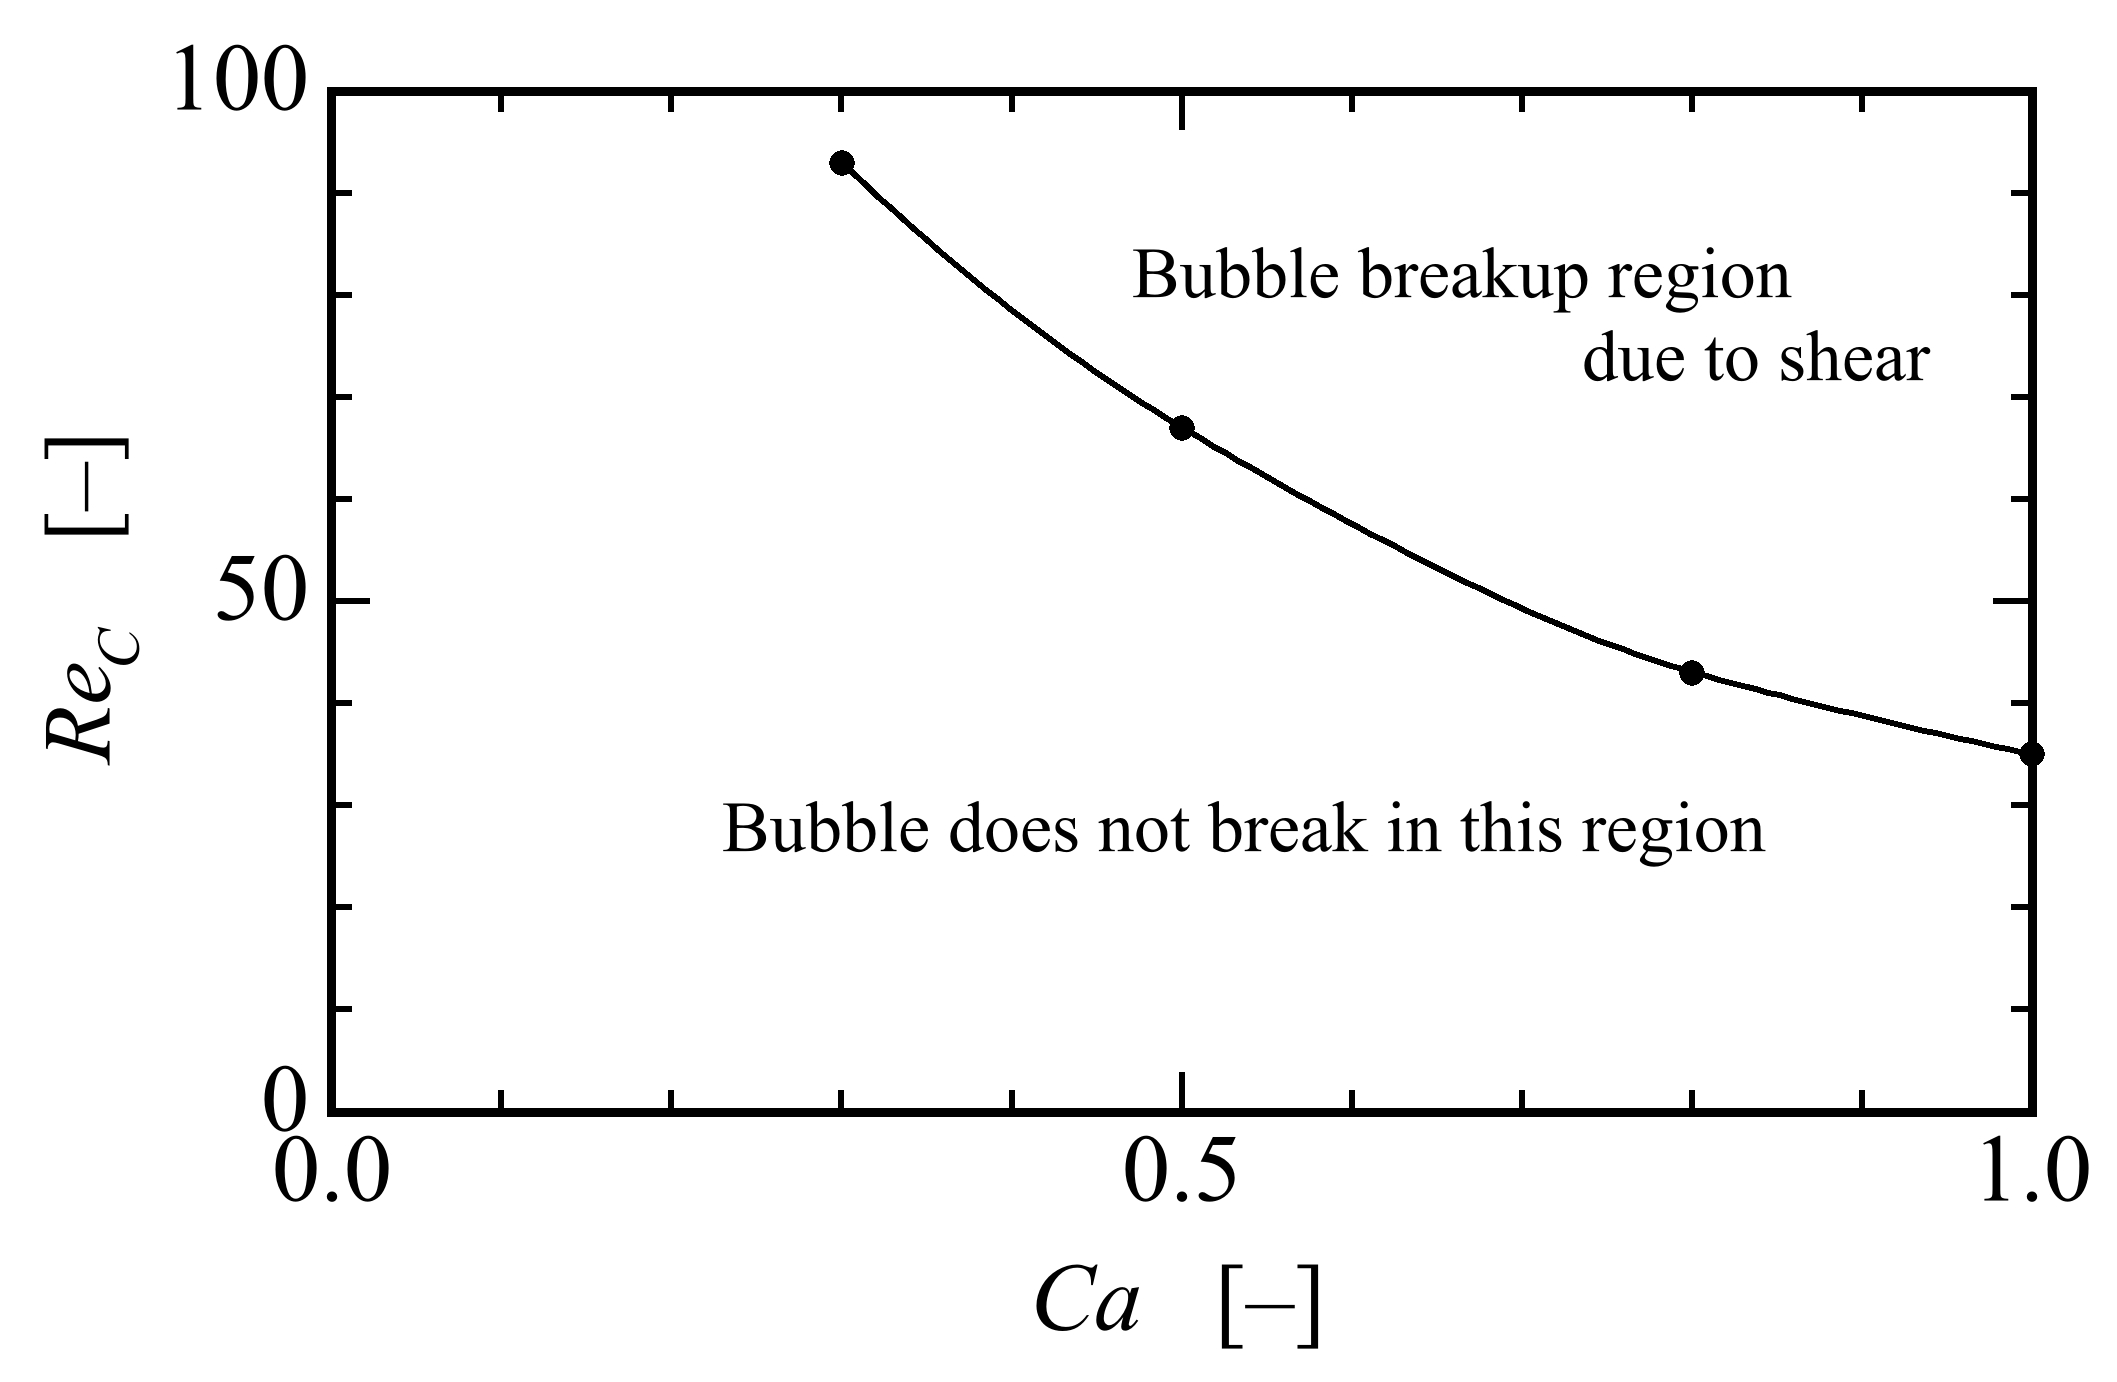
\includegraphics[width=\textwidth]{Fig12-Critical-Re}
  \caption{A plot of the critical Reynolds number versus Capillary number
	for the data listed in Table \ref{tab:CaRecComparison}.  The
	linear least squares best fit for the $\log(Re_{c})$ is
	$\log(Re_{c})=4.9-1.41(Ca)$ (i.e. $Re_{c}=138.3 e^{-1.41 Ca}$)
	with a predicted variance
	for the parameters ``$4.9$'' and ``$-1.41$'' being
	$4.2E-3$ and $8.4E-3$ respectively.  Even for the
	given data that we computed, it is suggested that 
	a ``bubble break-up map''
	can be derived, in which for the conditions that
	$\lambda$ = $\eta$ = 1.0 $\times$ $10^{-3}$, $0.3<Ca<1$, and
        the initial/boundary conditions are given by (\ref{IC_BC}),	
	one
	can predict whether a given $(Ca,Re)$ pair will result in shear
	induced bubble break-up or not.  
	   }
  \label{fig:CaRecFit}
\end{figure}
%

%  -----------------------------------------------------------------------------
\section{Conclusions}
%  -----------------------------------------------------------------------------
The bubble deformation and breakup process in simple linear shear flow liquid
was explored numerically using the CLSVOF computational method.  In this study,
the critical Reynolds number $Re_{c}$, at which bubble breakup first occurs,
was determined for several flow conditions, and the differences between bubble
deformation and breakup were compared with the well-known analogous process of
drop deformation and breakup.

Numerical results revealed significant differences between bubble deformation
and breakup and the corresponding drop dynamics.  For case of bubble, it was
discovered that much stronger shear flows are necessary to induce interface
breakup compared with a drop immersed in a similar flow field.  That is, a much
larger Reynolds number flow is required in order to induce bubble breakup.  The
behavior of bubble breakup was very similar through the $Ca$ number range
considered in our computations: the bubble underwent a similar breakup
mechanism in which rupture occurred at a thread-bridge part that followed a
doglegged shape formation stage.  In bubble deformation without breakup, near
$Re_{c}$, the bubble did not maintain a stable deformed shape, in contrast to
drop deformation near the critical Reynolds number.  The bubble exhibited
pronounced underdamped behavior: the bubble oscillated between elongating and
shrinking motions for non-rupturing flow conditions.

We attribute the large differences in morphology for the bubble undergoing
breakup, compared with the drop, to the density and viscosity ratio.  The
density and viscosity ratio remarkably impacts on bubble/drop deformation and
breakup.  The bubble deformation and breakup is subject to a synergistic
coupling of the density and viscosity ratio, and whose effect will be examined
separately in future work.


%\bibliography{apssamp}% Produces the bibliography via BibTeX.
\bibliography{references}

%  -----------------------------------------------------------------------------
%  -----------------------------------------------------------------------------
\end{document}
%
% ****** End of file apssamp.tex ******
